\documentclass{article}

% Language setting
% Replace `english' with e.g. `spanish' to change the document language
\usepackage[english]{babel}

% Set page size and margins
% Replace `letterpaper' with`a4paper' for UK/EU standard size
\usepackage[a4paper,top=2cm,bottom=2cm,left=3cm,right=3cm,marginparwidth=1.75cm]{geometry}

% Useful packages
\usepackage{amsmath}
\usepackage{fullpage}
\usepackage{amssymb}
\usepackage{amsthm}
\usepackage{bbm}
\usepackage{graphicx}
\usepackage{csquotes}
\usepackage[colorlinks=true, allcolors=blue]{hyperref}
\usepackage[style=alphabetic-verb]{biblatex}
\addbibresource{references.bib}

\newtheorem{definition}{Definition}
\newtheorem{theorem}{Theorem}[section]
\newtheorem{lemma}[theorem]{Lemma}
\newtheorem{corollary}[theorem]{Corollary}
\newtheorem{remark}[theorem]{Remark}










\title{Graphical Nadaraya Watson estimator}
\author{Martin Gjorgjevski}
\date{May 2022}
\DeclareMathOperator\supp{supp}
 \DeclareMathOperator{\LPM}{LPM}
 \DeclareMathOperator\dummy{dummy}

\usepackage{microtype}

\begin{document}

\maketitle
\begin{abstract}
The topic of this report is a mixture of nonparametric staitstics and random graph theory.
We analyze a simple and intuitive estimator in a graph regression setting. Given observations associated to a subset of the nodes, the estimator simply averages the observations over the neighbours of the node in question. We consider the latent position random graph model where each node $i$ is associated to an unobserved random point $X_i$, these points being i.i.d. variables which take values in $\mathbb{R}^d$. Edges  occur independently (conditionally on the latent positions), with the probability  that nodes  $i$ and $j$ are connected by an edge equal to $k(X_i,X_j)$ where $k$ is a kernel on $\mathbb{R}^d$. While such an assumption on the data generating process may be an oversimplification for practical applications, it is a useful playground for a theoretical  understanding quantities such as sample complexities and generalization bounds.
Due to the connection with the classical Nadaraya Watson kernel based estimator, we call the proposed estimator the Graphical Nadaraya Watson estimator, denoted by $\hat{f}_{GNW}(x)$. In the nonparametric estimation literature it is well known that convolutional kernels need bandwith adaptation in order to achieve optimal performance, while in the graph learning literature it is well known that large social networks observed in practice are sparse (in terms of the adjacency matrix). In our setting we show that under certain conditions on $k$, these two phenomena are closely related. We show that for bounded functions $f$, $Var(\hat{f}_{GNW}(x))=\Theta(1/\deg(x))$ and for bounded and sufficiently smooth functions $f$ the mean square error of $E(\hat{f}_{GNW}(x)-f(x))^2=O(\max(1/deg(x),deg(x)/n))$. As a consequence we conclude that the Graphical Nadaraya Watson estimator is consistent for arbitrarily sparse graphs. On the other hand, $\hat{f}_{GNW}$ suffers from the problems common in statstics such as bias-variance trade-off and the curse of dimensionality. Despite the simplicity of $\hat{f}_{GNW}$, we believe that these results will contribute to improve the theoretical understanding of more sophisticated graph learning architectures  such as Graph Neural Networks (GNNs). 
\end{abstract}



\tableofcontents




\section{Introduction}
\subsection{Nonparametric regression and the Nadaraya-Watson estimator}


\paragraph{Nonparametric regression} In the classical nonparametric regression problem  we are given data points  $X_1,...,X_n\in\mathbb{R}^d$ which are either fixed\footnote{For example equally spaced points on the unit cube $[0,1]^d$} or independent samples with common density $p$ and  
noisy observations $Y_i=f(X_i)+\epsilon_i$. Here,  $f\colon\mathbb{R}^d\to\mathbb{R}$ is an unknown function and in some suitable function class   $\mathcal{F}$ and
$\epsilon_1,...,\epsilon_n$ are assumed to be i.i.d. centered variables with variance $\sigma^2$. The goal is to estimate $f$. The term \textit{nonparametric} stems from the fact that the function class $\mathcal{F}$ can not be parametrized by a  subset of $\mathbb{R}^m$ for any $m\in \mathbb{N}$.

\paragraph{The Nadaraya Watson estimator} A kernel $k$ on $\mathbb{R}^d$ is a symmetric function $k:\mathbb{R}^d\times\mathbb{R}^d\rightarrow \mathbb{R}$. The kernel $k$ is said to be positive semi definite if for any $x_1,...,x_n\in\mathbb{R}^d$, and the $n\times n$ matrix with $(i,j)$-th entry $k(x_i,x_j)$ is positive semi definite. If there exists a function $K\colon\mathbb{R}^d\to\mathbb{R}$ such that for all $x,y\in\mathbb{R}^d$, $k(x,y)=K(x-y)$ then $k$ is said to be a stationary kernel. If, in addition, for all $x,y\in\mathbb{R}^d$, $k(x,y)=K(||x-y||)$ then $k$ is said to be a radial basis kernel. The idea behind the Nadaraya Watson estimator is to \textit{choose} a stationary kernel $k$ and a bandwith parameter $h>0$ and to estimate $f$ by

\begin{equation}
\label{NW_def}
    \hat{f}_{NW}(x)=\begin{cases}
    \frac{\sum_{i=1}^nY_ik(\frac{x-X_i}{h})}{\sum_{i=1}^n{k(\frac{x-X_i}{h}})} \quad &\text{if}\, \sum_{i=1}^n 
    k(\frac{x-X_i}{h})\neq 0\\
    0 \quad &\text{otherwise}\\
    \end{cases}
\end{equation}
The quality of the estimator in terms of the $L^2$-risk $E(\hat{f}_{NW}(x)-f(x))^2$ at a fixed point $x\in\mathbb{R}^d$ will depend on the many factors, such as the regularity of $f$, the choice of the kernel $k$ but most importantly on the choice of bandwith $h>0$. The $L^2$-risk admits the bias-variance decomposition

\begin{equation}
\label{eqn:bias-variance-decomp}
E(\hat{f}_{NW}(x)-f(x))^2=Var(\hat{f}_{NW}(x))+(E\hat{f}_{NW(x)}-f(x))^2
\end{equation}
The quantity $E(\hat{f}_{NW}(x)-f(x))$ is known as bias and under regularity assumptions on $f$ such as $\alpha$-Holder continuity, this term is upper bounded by $Ch^{\alpha}$ where $C$ depends on $k$ and $\alpha$ but not on the sample size $n$. We will give a more thorough discussion of the bias in Chapter 4. On the other hand, the variance $Var(\hat{f}_{NW}(x)$ tends to increase as $h$ decreases, this is the famous bias-variance tradeoff phenomenon. In the fixed design setting optimal rates for $h$ are available, and they are dependent on the sample size $n$ (see \cite{Tsybakov} section 1.5 and section 1.6, Proposition 1.13). The main takeaway is that the statistician should adapt $h$ with respect to the sample size $n$. 

\paragraph{Linear estimators}
A general class of estimators have been extensively studied in the literature both theoretically and empirically is the class of linear estimators. A linear nonparametric regression estimator for $f$ is an estimator $\hat{f}$ which can be expressed as $\hat{f}(x)=\sum_{i=1}^nY_iW_{n,i}(x)$ where $W_{n,i}(x)$ depends on $x,X_1,...,X_n$ but not on the observations $Y_1,...,Y_n$. For this class of estimators one typically takes $\mathcal{F}$ to be a Holder or a Sobolev space over a region $G\subseteq \mathbb{R}^d$. One generalization of the Nadaraya Watson estimator when $d=1$ are the local polynomial estimators which aim to estimate not only $f$ but also several of its derivatives $f^{(1)},...,f^{(l)}$. Another popular type of linear estimators are the projection estimators. They assume that $f$ belongs in a the span\footnote{potentially closed linear span} of a certain basis and then  try to estimate coefficients with respect to said basis (e.g. trigonometric basis, wavelets and  splines among others). 
\subsection{Random graphs and Latent Position Models}

\paragraph{The Erdos-Renyi Model}

The most well known random graph model is the Erdos-Renyi random graph $G(n,p)$, for positive integer $n$ and $0\leq p\leq 1$. This model samples a random graph on $n$ vertices with edges between vertices appearing independently with probability $p$. Results about $G(n,p)$ are stated  asymptotically, that is as $n\to\infty$, for a certain range of values of $p$ (more often than not depending on $n$), a graph sampled from $G(n,p)$ has a certain property with overwhelming probability. In their pioneering work, Erdos and Renyi show that for many graphical properties there is a sharp treshold $p_c$ in the sense that for $p>p_c$ almost all $G(n,p)$ graphs have the property, while for $p<p_c$ almost none of them have the property. Classical examples are $p_c=1/n$ for the emergence of the giant component and $p_c=\log(n)/n$ for connectedness. 


\paragraph{Large Graphs from Real World Data}

Many large complex networks in the real world such as the World Wide Web, Movie actor collaboration networks, Citation Networks to name a few, have properties which are not present in the Erdos-Renyi graph. When such networks were compared to Erdos Renyi Random graph with same number of nodes and same average degree, it is observed that cliques in the Real World Networks form more often than in their Erdos-Renyi have  counterpart, Similarly, Real World Networks have degree distributions which typically obey a power law, i.e. the proportion of vertices which have degree $k$ is of the order $k^{-\alpha}$, while for their Erdos-Renyi model counterpart this should be a Poisson distribution. Such observations prompted the scientific community to consider different models for the data generating process which can better explain these phenomena (\cite{Albert}, Section 2).  

\paragraph{The Stochastic Block Model} The Stochastic Block Model of Holland and Leindhart (\cite{Holland1983StochasticBF}) naturally includes clustering of vertices. It assumes that $n$ vertices are randomly sampled from $K$
communities, and that conditionally on these communities edges form independently with probability depending only on the communities. More formally, $SBM(n,p,W)$ where $n$ is a positive integer, $p=(p_1,...,p_K)$ is $K$ dimensional vector with $0\leq p_l\leq 1$ and $\sum_{l=1}^Kp_l=1$ and $W$ is a $K\times K$ symmetric matrix with entries $0\leq w_{i,j}\leq 1$ generates edges on vertices $[n]$ by first randomly assigning a community $C_1,...,C_K$ to each node with $P(i\in C_l)=p_l$ (these assignments are independent over distinct vertices) and then generating edges depending on the community of the endpoints of the edge, that is $P(i\sim j| i\in C_l,j\in C_s)=w_{ls}$. There are several questions in the $SBM$ model such as deciding if an observed graph is indeed sampled by an $SBM$, under which conditions is there a way to fully or partially recover communities based on a single observed graph. The Stochastic Block Model has a long history in the statistics literature (  \cite{Snijders}). For recent developments we refer to (\cite{Abbe}).

\paragraph{The Random Geometric Graph} Another popular random graph model is the Geometric Random Graph, which is generated by sampling $n$ independent random variables $X_1,...,X_n\in\mathbb{R}^d$ and placing edges between nodes if the sampled points are sufficiently close, that is there is $h>0$ such that $P(i\sim j)=I(||X_i-X_j||\leq h)$. The value $h$ controls how well connected the graph is, in the sense that smaller values of $h$ give rise to sparser graphs. It is common to study how the behavior of certain graph statistics (such as degree distributions, average degrees and  subgraph counts) changes with respect to $h$. A classical treatment of this topic is the Monograph of Penrose (\cite{Penrose2003RandomGG})
.

\begin{figure}
    \centering
    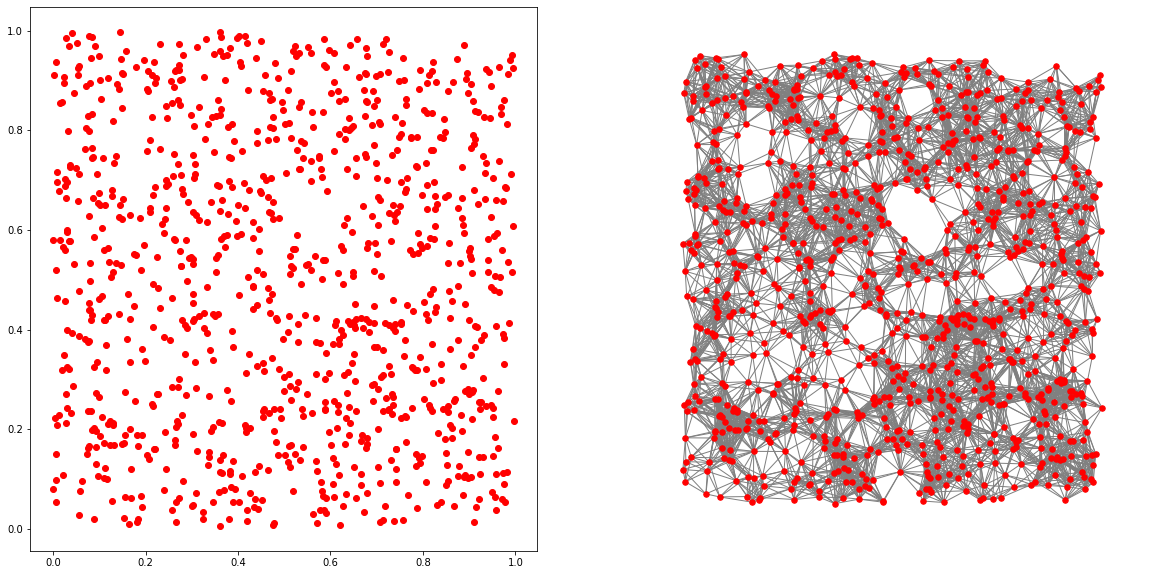
\includegraphics[width=0.75\textwidth]{sparse_rgg.png}
    \caption{Random Geometric Graph with $n=1000$ uniformly sampled points, $h=\sqrt{\frac{\log(n)}{n}}$}
    \label{Rgg_fig}
\end{figure}

\paragraph{Latent Position Models} The Latent Position Model was introduced by (\cite{Hoff}).
For a positive integer $n$, a  kernel $k$ on $\mathbb{R}^d$ taking values between $0$ and $1$ and a density $p$ on $\mathbb{R}^d$ the Latent Position Model $\LPM(n,k,p)$ generates edges between vertices of $[n]$ in two stages; first a sample of size $n$ of i.i.d. variables $X_1,...,X_n$ with density $p$ is drawn. The variable $X_i$ can be thought of as the position of node $i$ in the latent space. Next, given the sample $(X_1,...,X_n)$ edges are drawn independently with $P(i\sim j|X_i,X_j)=k(X_i,X_j)$. Intuitively this means that we are more likely to observe an edge between two nodes which have positions that are similar with respect to $k$. Both the Stochastic Block Model and the Random Geometric Graph can be thought of as a Latent Position Models with a suitable kernel $k$. If the kernel $k$ is stationary then the graph structure of the $LPM$ is in many respects similar to the graph structure of the Random Geometric Graph. On the other hand, The Stochastic Block Model can be represented as a Latent Position Model with $d=1$, with a kernel $k$ which can classify points that are arbitrarily close as being dissimilar. For the purposes of regression, the case where the kernel $k$ is stationary is a much more natural setup.

\begin{figure}[h!]
    \centering
    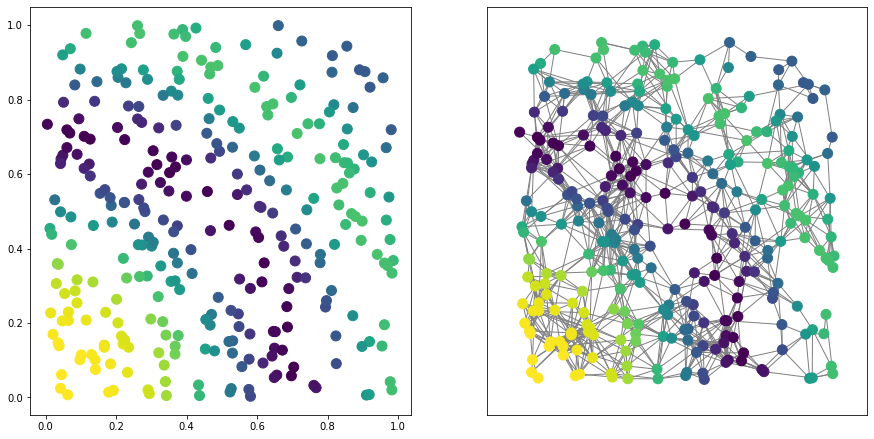
\includegraphics[width=0.75\textwidth]{lpm_image_correct.png}
    \caption{Latent position model with $n=300$ nodes, Gaussian kernel, and bandwith $h=0.75(\frac{\log(n)}{n})^{1/2}$}
    \label{fig:LPM_plot}
\end{figure}



\subsection{Framework}

\paragraph{Framework} We observe a random graph with vertex set $[n+1]$  sampled according to an $\LPM(n+1,k_n,p)$ and assume that for nodes $i=1,...n$ (all but the last node) there is a label of the form $Y_i=f(X_i)+\epsilon_i$ with $f\colon\mathbb{R}^d\to\mathbb{R}$. Besides the graph itself and the explanatory variables $Y_1,...,Y_n$ no other quantities are assumed to be known. We write $X$ in place of $X_{n+1}$ and for $i=1,...,n$ we write $a(X,X_i)$ for the indicator that there is an edge between the node $n+1$ and node $i$. To describe edge generation more precisely, we assume that for $i=1,...,n$ the indicator of an edge between $X$ and $X_{i}$ is given by 

\begin{equation*}
    a(X,X_{i})=I(U_i\leq k(X,X_i))
\end{equation*}
where $U_1,...,U_n$ are uniform variables on $[0,1]$, such that $(U_1,...,U_n,X_1,...,X_n,X,\epsilon_1,....,\epsilon_n)$ are jointly independent variables. 

For $x\in\mathbb{R}^d$, we define

\begin{equation*}
    a(x,X_i)=I(U_i\leq k(x,X_i))
\end{equation*}

We introduce the \textbf{Graphical Nadaraya Watson} estimator given by 
\begin{equation}
\label{gnw_def}
\hat{f}_{GNW}(x)=\begin{cases}
    \frac{\sum_{i=1}^n Y_ia(x,X_i)}{\sum_{i=1}^n a(x,X_i)} \quad &\text{if}\, \sum_{i=1}^n a(x,X_i)\neq 0\\
    0 \quad &\text{otherwise}\\
\end{cases}
\end{equation}
We are interested in two types of risk which we consider as the main measure of performance of $\hat{f}_{GNW}(x)$.


\begin{itemize}
    \item For a fixed point $x\in\supp{p}$, we are interested in a bound on the risk at the point $x$ given by
\begin{equation}
\label{fixed_point_risk}
    E(\hat{f}_{GNW}(x)-f(x))^2
\end{equation}
    \item For the random variable $X$ which represents node $n+1$ we define the risk at the random point $X$

\begin{equation}
\label{random_point_risk}
    E(\hat{f}_{GNW}(X)-f(X))^2
\end{equation}
\end{itemize}

To our knowledge there are no results in on graph regression in this context.


\subsection{Expected local degrees}
We introduce the quantity 
\begin{equation}
\label{c_n_eqn}
    c_n(x)=\int_{\mathbb{R}^d} k_n(x,z)p(z)dz
\end{equation}
Heuristically speaking, when conditioned on $X=x$ the degree of $X$ is
$\sum_{i=1}^n a(x,X_i)$. Hence we define the expected local degree at $x$ with

\begin{equation}
\label{local_degree}
    d_n(x)=nc_n(x)
\end{equation}

\subsection{Classical and Graphical Nadaraya Watson estimators: similarities and differences}

Because of the kernel based data generating process in the Latent position model, the Graphical Nadaraya Watson Estimator has strong connections with the classical Nadaraya Watson estimator. We emphasize the fact that while in classical nonparametric estimation the choice of the kernel is up to the statistician, in our setup the kernel $k_n$ is given with the Latent Position Model, and hence it represents an oracle quantity. We define the integral operator $T_{k_n}(\cdot,x)$ on the set of bounded functions  $f\colon\mathbb{R}^d\to\mathbb{R}$ by
\begin{equation}
\label{T_n_eqn}
    T_k(f,x)==\int_{\mathbb{R}^d}f(z)k_n(x,z)p(z)dz
\end{equation}
It is easy to see that 
\begin{equation}
    T_{k_n}(f,x)=Ef(X_i)a(x,X_i)
\end{equation}
Note also that $c_n(x)=T_{k_n}(1,x)$.
As a rough heuristic\footnote{If $k_n$ did not depend on $n$ this heuristic would be a fact, due to the law of large numbers} to motivate further discussion, we expect that $\frac{1}{n}\sum_{i=1}f(X_i)a(x,X_i)-T_{k_n}(f,x)\to 0$. As $\hat{f}_{GNW}(x)$ is a quotient of $\frac{1}{n}\sum_{i=1}^n Y_ia(x,X_i)$ and $\frac{1}{n}\sum_{i=1}^na(x,X_i)$
which are close to $T_{k_n}(f,x)$ and $c_n(x)$ respectively, it is reasonable to expect that $\hat{f}_{GNW}(x)$ will be close to

\begin{equation}
    b_n(f,x)=\frac{T_{k_n}(f,x)}{c_n(x)}
\end{equation}
Note that the same rough heuristic applies to the classical Nadaraya Watson estimator by replacing $a(x,X_i)$ by $k_n(x,X_i)$.

\subsection{Strategy}

The risk at the point $x$ (\ref{fixed_point_risk}) is much easier to control compared to the risk at the random point $X$ (\ref{random_point_risk}), so first we give the main ideas on how to bound (\ref{fixed_point_risk}) from above. The strategy is to decompose Equation (\ref{fixed_point_risk}) into a variance term

\begin{equation}
\label{variance_term}
E(\hat{f}_{GNW}(x)-b_n(f,x))^2
\end{equation}
and a bias term
\begin{equation}
\label{bias_term}
b_n(f,x)-f(x)
\end{equation}
and bound those terms separately. The tools used to the variance term (\ref{variance_term}) are probabilistic in nature such as decoupling arguments and concentration inequalities. On the other hand the tools needed  to bound the bias term (\ref{bias_term}) are of geometric nature, as they basically ammount to studying convergence of certain integral operators towards the identity. We will show that in a general Latent position model the variance term (\ref{variance_term}) satisfies

\begin{equation*}
    \frac{C_1(\sigma^2)(1-e^{-d_n(x)})}{d_n(x))}\leq E(\hat{f}_{GNW}(x)-b_n(f,x))^2\leq \frac{C_2(B,\sigma^2)}{d_n(x})
\end{equation*}
where $d_n(x)$ is the local average degree given by Equation (\ref{local_degree}). On the other hand the bias in a general Latent position model may behave poorly. We will restrict our attention to the geometric setting where the kernel $k_n$ is of the form $k_n(x,z)=\rho_n\frac{K(x-z}{h_n}$ which will mimic the properties of the Random Geometric Graph. Pointwise results in this setting are still easy to obtain. Finally, once we establish upper bounds on Equation (\ref{bias_term}) and (\ref{variance_term}) we may integrate them against the $p$ to obtain bounds for the risk at the random point $X$. This strategy requires strong assumption on the distribution in order to work.  

\paragraph{Outline}

\section{Bounding the variance at a point}
\subsection{Computing  $E\hat{f}_{GNW}(x)$}
The risk at the point $x$ (\ref{fixed_point_risk}) admits the decomposition
\begin{equation}
\label{eqn_bias_variance}
    E(\hat{f}_{GNW}(x)-f(x))^2=Var(\hat{f}_{GNW}(x))+(E\hat{f}_{GNW}(x)-f(x))^2
\end{equation}
Equation (\ref{eqn_bias_variance}) is known as the bias-variance decomposition of risk. If we want asymptotically vanishing risk at the point $x$, i.e. 
$E(\hat{f}_{GNW}(x)-f(x))^2\rightarrow 0$ as $n\rightarrow\infty$, we need  $E(\hat{f}_{GNW}(x))\rightarrow f(x)$ as $n\rightarrow\infty$. Thus it is of basic interest to compute $E(\hat{f}_{GNW}(x))$, at least asymptotically. Being a quotient of two random variables, the exact value of 
$E\hat{f}_{GNW}(x)$ may seem difficult to compute. 
In this section we compute explicitly  $E\hat{f}_{GNW}(x)$ for all $x$ such that $c_n(x)>0$. This is done via a decoupling argument. The method used here will be used again to bound the risk at the point $x$.

\paragraph{Decoupling argument}

Let $I\subseteq [n]$.
For $I=\emptyset$ we define

\begin{equation}
\label{eqn_R_empty}
R_{\emptyset}(x)=\begin{cases}
    \frac{1}{\sum_{i=1}^n a(x,X_i)} \quad &\text{if}\, \sum_{i=1}^n a(x,X_i)>0\\
    0 \quad &\text{otherwise}\\
\end{cases}
\end{equation}
 and for $I\subseteq [n]$, $I\neq\emptyset$ we define  
\begin{equation*}
    R_I(x)=\frac{1}{|I|+\sum_{j\notin I}a(x,X_j)}
\end{equation*}
For convenience of notation we write $R_i(x)=R_{\{i\}}(x)$.
Note that for all pairs of disjoint subsets $I,J\subseteq [n]$ we have

\begin{equation}
\label{eqn_R}
R_J(x)\prod_{i\in I}a(x,X_i)=R_{I\cup J}(x)\prod_{i\in I}a(x,X_i)
\end{equation}
and $R_{I\cup J}(x)$ is independent from $\{a(x,X_i)|i\in I\}$. In the special case when $I=\{i\}$ and $J=\emptyset$, Equation (\ref{eqn_R}) becomes  

\begin{equation}
\label{eqn_R_single}
R_{\emptyset}(x)a(x,X_i)=R_{i}(x)a(x,X_i)
\end{equation}
This simple observation makes the computation of $E\hat{f}_{GNW}(x)$  possible.
\begin{lemma}
\label{lemma_exp}
For all $i-1,2,...,n$ we have
\begin{equation*}
    ER_i(x)=\frac{1-(1-\frac{d_n(x)}{n})^n}{d_n(x)}
\end{equation*}
\end{lemma}
\begin{proof}
Note that $R_i(x)$, $i=1,2,...,n$ are identically distributed, hence  $ER_i(x)=ER_1(x)$ for $i=2,...,n$.
By summing Equations (\ref{eqn_R_single}) for $i=1,2,3,...,n$ we have 
\begin{equation}
\label{eqn_for_Ri}
    \sum_{i=1}^n a(x,X_i)R_i(x)=R_{\emptyset}(x)\sum a(x,X_i)=I(\sum_{i=1}^n a(x,X_i)>0)
\end{equation}
Taking expectation and using the fact that $R_i(x)$ and $a(x,X_i)$ are independent, we get

\begin{equation}
\label{eqn_for_ERi}
\begin{split}
    E(\sum_{i=1}^n a(x,X_i)R_i(x))&=\sum_{i=1}^n E(a(x,X_i)R_i(x))\\
    &=\sum_{i=1}^n E(a(x,X_i))ER_i(x)\\
    &=nc_n(x)ER_1(x)
\end{split}
\end{equation}
On the other hand,
\begin{equation}
\label{eqn_for_Rempty}
    P(\sum_{i=1}^n a(x,X_i)>0)=1-P(\sum_{i=1}^n a(x,X_i)=0)=1-(1-c_n(x))^n
\end{equation}

The result follows by combining Equations (\ref{eqn_for_Ri}), (\ref{eqn_for_ERi}) and (\ref{eqn_for_Rempty}).

\end{proof}

\begin{corollary}
\label{expectation_comp}
\begin{equation*}
    E\hat{f}_{GNW}(x)=b_n(f,x)(1-(1-c_n(x))^n)
\end{equation*}
\end{corollary}
\begin{proof}

By Equation (\ref{eqn_R}) we have

\begin{equation*}
    \hat{f}_{GNW}(x)=\sum_{i=1}^n Y_ia(x,X_i)R_i(x)
\end{equation*}

Hence, taking expectation and using Lemma  \ref{lemma_exp}, we get 

\begin{equation*}
\begin{split}
    E\hat{f}_{GNW}(x)&=\sum_{i=1}^nEY_ia(x,X_i)R_i(x)\\
    &=\sum_{i=1}^nEY_ia(x,X_i)ER_i(x)\\
    &=nEY_1a(x,X_1)ER_1(x)\\
    &=\frac{T_{k_n}(f)(x)(1-(1-c_n(x))^n)}{c_n(x)}\\
    &=b_n(f,x)(1-(1-c_n(x))^n)
\end{split}
\end{equation*}

\end{proof}



\subsection{The decoupling argument}
In the previous section we found an explicit expression for $E\hat{f}_{GNW}(x)$ (Corollary \ref{expectation_comp}). While this makes computation of $Var(\hat{f}_{GNW}(x))=E(\hat{f}_{GNW}(x)-E\hat{f}_{GNW}(x))^2$ possible, we find that it is much simpler to analyse $E(\hat{f}_{GNW}(x)-b_n(f,x))^2$ instead. Note that by definition

\begin{equation}
\label{gnw_no_edges}
    I(\sum_{i=1}^na(x,X_i)=0)\hat{f}_{GNW}(x)=0
\end{equation}
or equivalently
\begin{equation}
\label{gnw_edges}
   I(\sum_{i=1}^na(x,X_i)>0)\hat{f}_{GNW}(x)=\hat{f}_{GNW}(x) 
\end{equation}
Thus 

\begin{equation}
\label{variance_decomp}
\begin{split}
    E(\hat{f}_{GNW}(x)-b_n(f,x))^2&=E[(\hat{f}_{GNW}(x)-b_n(f,x))^2I(\sum_{i=1}^na(x,X_i)>0))]\\
    &+E[(\hat{f}_{GNW}(x)-b_n(f,x))^2I(\sum_{i=1}^na(x,X_i)=0)]\\
    &=E(\hat{f}_{GNW}(x)-b_n(f,x)I(\sum_{i=1}^na(x,X_i)>0))^2+b_n^2(f,x)P(\sum_{i=1}^na(x,X_i)=0)
\end{split}
\end{equation}
Using Equation (\ref{eqn_R}) and Equation (\ref{eqn_for_Ri}) we have
\begin{equation}
    \hat{f}_{GNW}(x)-b_n(f.x)I(\sum_{i=1}^n a(x,X_i)>0)=\sum_{i=1}^n(Y_i-b_n(f,x))a(x,X_i)R_i(x)
\end{equation}
In Lemma \ref{trick_lemma_pt_1} we show that the summands in this representation are uncorrelated and consequently obtain tractable expression for $E(\hat{f}_{GNW}(x)-b_n(f.x)I(\sum_{i=1}^n a(x,X_i)>0))^2$. In contrast, computing the variance $Var(\hat{f}_{GNW}(x))$ directly  leaves a much more complicated expression.

\begin{lemma}
\label{trick_lemma_pt_1}

\begin{equation*}
    E(\hat{f}_{GNW}(x)-b_n(f,x)I(\sum_{i=1}^n a(x,X_i)>0))^2=
    n[E(f(X_1)-b_n(f,x))^2a(x,X_i)+\sigma^2c_n(x)]ER_1^2(x)
\end{equation*}

\end{lemma}
\begin{proof}
Using Equation (\ref{eqn_for_Ri}), we have

\begin{equation}
\label{tricky_eqn}
\begin{split}
    E(\hat{f}_{GNW}(x)-b_n(f,x)I(\sum_{i=1}^na(x,X_i)>0))^2&=E(\sum_{i=1}^n(Y_i-b_n(f,x))a(x,X_i)R_i(x))^2\\
    &=\sum_{i=1}^n E(Y_i-b_n(f,x))a(x,X_i)R_i(x))^2\\
    &+\sum_{i\neq j}E((Y_i-b_n(f,x))(Y_j-b_n(f,x))a(x,X_i)a(x,X_j)R_i(x)R_j(x))
\end{split}
\end{equation}
For $i\neq j$, using Equation (\ref{eqn_R}), together with the fact that $R_{i,j}(x)$ is independent from  $Y_i,Y_j,a(x,X_i)$ and $a(x,X_j)$, as well as the fact that the pairs $(Y_i,a(x,X_i)$ and $(Y_j,a(x,X_j)$ are independent, we have 

\begin{equation}
\label{dr_trick}
\begin{split}
    &E[(Y_i-b_n(f,x))(Y_j-b_n(f,x))a(x,X_i)a(x,X_j)R_i(x)R_j(x)]=\\
    &E[(Y_i-b_n(f,x))(Y_j-b_n(f,x))a(x,X_i)a(x,X_j)R_{i,j}^2(x)]=\\
    &E[(Y_i-b_n(f,x))a(x,X_i)]E[(Y_j-b_n(f,x)a(x,X_j))]ER_{i,j}^2(x)=0
\end{split}
\end{equation}

Furthermore,
\begin{equation}
\label{sr_trick}
\begin{split}
    \sum_{i=1}^n E[(Y_i-b_n(f,x)^2a(x,X_i)R_i^2(x)]&=\sum_{i=1}^n E((Y_i-b_n(f,x))^2a(x,X_i)ER_i^2(x)\\
    &=nE[((Y_1-b_n(f,x))^2a(x,X_i)]ER_1^2(x)\\
    &=n[E(f(X_1)-b_n(f,x))^2a(x,X_i)+\sigma^2c_n(x)]ER_1^2(x)
\end{split}
\end{equation}


\end{proof}
\subsection{Lower bounds}
We show that the presence of noise alone is sufficient for a lower bound of $E(\hat{f}_{GNW}(x)-b_n(f,x))^2$ that is of order $\frac{1}{d_n(x)}$.  
\begin{lemma}
\label{variance_lower_bound}
\begin{equation*}
    E(\hat{f}_{GNW}(x)-b_n(f,x))^2\geq \frac{\sigma^2(1-e^{-d_n(x)})^2}{d_n(x)}
\end{equation*}

\end{lemma}

\begin{proof}
By Equation (\ref{variance_decomp}), Lemma
\ref{expectation_comp}, Lemma  
\ref{trick_lemma_pt_1} and the basic inequality  $1-t\leq e^{-t}$ valid for all $t\geq 0$, we have

\begin{equation}
\begin{split}
E(\hat{f}_{GNW}(x)-b_n(f,x))^2&\geq E(\hat{f}_{GNW}(x)-b_n(f,x)I(\sum_{i=1}^n a(x,X_i)>0))^2\\
&=n[E(f(X_1)-b_n(f,x))^2a(x,X_i)+\sigma^2c_n(x)]ER_1^2(x)\\
&\geq \sigma^2nc_n(x)ER_1^2(x)\\
&\geq \frac{\sigma^2(1-(1-c_n(x))^n)^2}{nc_n(x)}\\
&\geq \frac{\sigma^2(1-e^{-nc_n(x)})^2}{nc_n(x)}
\end{split}
\end{equation}

\end{proof}

\subsection{Upper bounds}

\begin{lemma} 
\label{trick_lemma_pt2}
For $n\geq 3$
\begin{equation*}
    E(\hat{f}_{GNW}(x)-b_n(f,x)I(\sum_{i=1}^n a(x,X_i)>0))^2\leq (4B^2+\sigma^2)(\frac{65}{d_n(x)})
\end{equation*}

\end{lemma}


\begin{proof}
Recalling Lemma \ref{trick_lemma_pt_1} and using the fact that $||f||_{\infty}\leq B$, we have 


\begin{equation}
\label{ubv_1}
     n[E(f(X_1)-b_n(f,x))^2a(x,X_i)+\sigma^2c_n(x)]ER_1^2(x)
     \leq (4B^2+\sigma^2)nc_n(x)ER^2_1(x)
\end{equation}

Hence it suffices to control $ER_1^2(x)$. We do this by splitting the expectation on the event that we observe at least $\frac{1}{2}(n-1)c_n(x)$ edges from $a(x,X_i)$, $i=2,...,n$ and on it's complement. Let 
\begin{equation}
    A(x)=\{\sum_{i=2}^na(x,X_i)\geq \frac{1}{2}(n-1)c_n(x)\}
\end{equation}

For $n\geq 2$ we have

\begin{equation}
\label{meat_good_part}
ER_1^2(x)I(A(x))\leq \frac{1}{(1+\frac{1}{2}(n-1)c_n(x))^2}P(A(x))\leq \frac{16}{n^2c_n^2(x)}
\end{equation}

An application of Bernstein's inequality for bounded distributions (\cite{vershynin} Theorem 2.8.4, page 39) with $a(x,X_i)-c_n(x)$, $i=2,3,...n$ as the bounded, centered and independent variables yields

\begin{equation}
\label{bernstein_result}
P(|\sum_{i=2}^{n}a(x,X_i)-(n-1)c_n(x)|\geq t)\leq 2\exp{(-\frac{t^2}{(n-1)c_n(x)(1-c_n(x))+\frac{t}{3}})}
\end{equation}
Setting $t=\frac{1}{2}(n-1)c_n(x)$ in Equation (\ref{bernstein_result}) together with the observation that $A^c(x)$ implies 

\begin{equation*}
    |\sum_{i=2}^{n}(a(x,X_i)-c_n(x))|\geq \frac{1}{2}(n-1)c_n(x)
\end{equation*}
For $n\geq 3$, we get

\begin{equation}
\label{meat_bad_part_anticip}
\begin{split}
    P(A^c(x))&\leq P(|\sum_{i=2}^{n}[a(x,X_i)-c_n(x)]|\geq \frac{1}{2}(n-1)c_n(x))\\
    &\leq \exp(-\frac{(n-1)c_n(x)}{4(1-c_n(x))+2/3})\\
    &\leq \exp(-\frac{3(n-1)c_n(x)}{14})\\
    &\leq \exp(-\frac{nc_n(x)}{7})
\end{split}
\end{equation}
Using the fact that $R_1\leq 1$ along with Equation (\ref{meat_bad_part_anticip}) we get

\begin{equation}
\label{meat_bad_part}
    ER^2_1(x)I(A^c(x))\leq P(A^c(x))\leq \exp(-\frac{nc_n(x)}{7})
\end{equation}

Combining Equation (\ref{meat_good_part}) and Equation (\ref{meat_bad_part}) gives

\begin{equation}
\label{meat}
ER^2_1(x)\leq \frac{16}{n^2c_n^2(x)}+\exp(-\frac{nc_n(x)}{7})
\end{equation}
The conclusion follows by combining Equationms (\ref{ubv_1}) and  (\ref{meat}), together with the basic inequality which states that for all $x\geq 0$, $x^2e^{-x}\leq 1$.
\end{proof}

\begin{lemma}
\label{variance_lemma}

\begin{equation*}
    E(\hat{f}_{GNW}(x)-b_n(f,x))^2\leq\frac{261B^2+65\sigma^2}{d_n(x)}
\end{equation*}
\end{lemma}

\begin{proof}

Using Equation (\ref{variance_decomp}),
Lemma \ref{trick_lemma_pt2} and using the basic inequality $1-t\leq \exp{(-t)}$ valid for all $t\geq 0$, we get

\begin{equation*}
\begin{split}
    E(\hat{f}_{GNW}(x)-b_n(f,x))^2
    &=E(\hat{f}_{GNW}(x)-I(\sum_{i=1}^na(x,X_i)b_n(f,x))^2+b_n^2(f,x)P(\sum_{i=1}^n a(x,X_i)=0)\\
    &\leq (4B^2+\sigma^2)(\frac{16}{nc_n(x)}+nc_n(x)\exp{(-\frac{nc_n(x)}{7})})+B^2(1-c_n(x))^n\\
    &\leq (4B^2+\sigma^2)(\frac{16}{nc_n(x)}+nc_n(x)\exp{(-\frac{nc_n(x)}{7})})+B^2\exp(-nc_n(x))
\end{split}
\end{equation*}
We conclude by using the basic inequalities:
for all $t\geq 0$, $t^2e^{-t}\leq 1$ and $te^{-t}\leq 1$.
\end{proof}

\begin{remark}
Suppose that $d_n(x)\to\infty$ as $n\to\infty$. Then Lemma (\ref{variance_lemma}) implies
\begin{equation*}
    E(\hat{f}_{GNW}(x)-b_n(f,x))^2\to 0
\end{equation*}
The growth of $d_n(x)$ can be arbitrarily slow, and the statement still holds. On the other hand if $d_n(x)\leq D$ for all $n\in\mathbb{N}$ and $\sigma^2>0$ then Lemma \ref{variance_lower_bound} gives 

\begin{equation*}
    E(\hat{f}_{GNW}(x)-b_n(f,x))^2\geq \frac{\sigma^2(1-e^{-D})}{D}>0
\end{equation*}

\end{remark}

\section{Controlling the Bias at a point}
\subsection{Geometric concerns}

\paragraph{Disconnected LPMs}

Since we want to consider the case where $X$ is a random variable, we need to make sure that $b_n(f,X)$ is well defined. In a general Latent position model it could happen that with positive probability for all $n\in\mathbb{N}$, $c_n(X)=0$, which means that with positive probability $X$ will be an isolated node in the graph. To avoid such trivialities 

\paragraph{Regularity}



\paragraph{Kernel assumptions}
These assumptions on $k_n$ in simple terms say that edge generation is dependent only on distances and thus make the model comparable to the Random Geometric Graph. It is an assumption so strong that it implies that  $dp(x)$-almost surely  $b_n(f,x)\rightarrow f(x)$ for a very general class of functions $f$. However, pointwise convergence of this form without uniform control of the error $|b_n(f,x)-f(x)|$ is not useful for our purposes. The following assumptions on $f$  
provide an easy way for bound on $\sup_{x\in\supp{p}}|b_n(f,x)-f(x)|$.
Finally, in order to translate our results for fixed points $x\in\supp{p}$ into results for a random variable $X$ with distribution $p$, we will need an assumption on the density $p$ itself.

\paragraph{Density assumptions}
\begin{itemize}
    \item $p\colon\mathbb{R}^d\to\mathbb{R}$ is $\beta$-Holder continous on it's support $\supp{p}$ i.e.
    there exists $L_{\beta}>0$ such that 
    
    \begin{equation*}
        \sup_{x,z\in\supp{p}} \frac{|p(x)-p(z)|}{||x-z||^{\beta}}\leq L_{\beta}  
    \end{equation*}
    
    
\end{itemize}

\begin{lemma}
\label{well_cond_lemma}
Suppose that \textbf{Kernel assumptions} hold. Then 

\begin{equation*}
    \supp{p}\subseteq \{x\in\mathbb{R}^d:c_n(x)>0\}
\end{equation*}
\begin{proof}
Suppose that $c_n(x)=0$. By continuity of $K$ at $0$, there is $r>0$ such that for all $z$ for which $||x-z||\leq rh_n$, $K(\frac{x-z}{h_n})\geq \frac{1}{2}$. Hence  

\begin{equation*}
\begin{split}
    \int I(||x-z||\leq rh_n) p(z)dz &\leq 2\int I(||x-z||\leq rh_n)K(\frac{x-z}{h_n})p(z)dz\\
    &\leq 2\int K(\frac{x-z}{h_n})p(z)dz\\
    &=2c_n(x)\\
    &=0
\end{split}
\end{equation*}
Hence $x\notin\supp{p}$, this proves the claim by contraposition.

\end{proof}


\end{lemma}

\begin{lemma}
\label{bias_control_lemma}

Suppose that \textbf{Kerenl assumptions} and \textbf{Function assumptions} hold. Then
    \begin{equation*}
    \sup_{x\in \supp(p)}|b_n(f,x)-f(x)|\leq L_{\alpha}M^{\alpha}h_n^{\alpha}
\end{equation*}
\end{lemma}

\begin{proof}
For $x\in\supp{p}$ by Lemma \ref{well_cond_lemma}, $c_n(x)>0$.
We have 

\begin{equation*}
\begin{split}
|b_n(f,x)-f(x)|&=|\frac{\rho_n\int f(z)K(\frac{x-z}{h_n})p(z)dz}{\rho_n\int K(\frac{x-z}{h_n})p(z)dz}-f(x)|\\
&=|\frac{\int f(z)K(\frac{x-z}{h_n})p(z)dz}{\int K(\frac{x-z}{h_n})p(z)dz}-\frac{\int f(x)K(\frac{x-z}{h_n})p(z)dz}{\int K(\frac{x-z}{h_n})p(z)dz}|\\
&=|\frac{\int[f(z)-f(x)]K(\frac{x-z}{h_n})p(z)dz
}{\int K(\frac{x-z}{h_n})p(z)dz}|\\
&\leq L_{\alpha}\frac{ \int 
||z-x||^{\alpha}K(\frac{x-z}{h_n})p(z)dz}{
\int K(\frac{x-z}{h_n})p(z)dz}\\
&\leq L_{\alpha}M^{\alpha}h_n^{\alpha}
\end{split}
\end{equation*}
Here, we used the fact that for any function $G\in L^1(dp(x))$, $\int_{\mathbb{R}^d} G(z)p(z)dz=\int_{\supp{p}} G(z)p(z)dz$ and crucially the facts that $f$ is $\alpha$-Holder continuous and that $K$ is compactly supported in the last inequality.
\end{proof}

\begin{corollary} Suppose that \textbf{Kernel assumptions} and \textbf{Function assumptions} hold. Let $X$ be a random variable with density $p$. 
\begin{equation*} 
P(|b_n(f,X)-f(X)|\leq L_{\alpha}M^{\alpha}h_n^{\alpha})=1
\end{equation*}

\end{corollary}
\begin{proof}
We have

\begin{equation*}
\begin{split}
    P(|b_n(f,X)-f(X)|\leq L_{\alpha}M^{\alpha}h_n^{\alpha})&=\int I(|b_n(f,x)-f(x)|\leq L_{\alpha}M^{\alpha}h_n^{\alpha})p(x)dx\\
    &\int_{\supp{p}} I(|b_n(f,x)-f(x)|\leq L_{\alpha}M^{\alpha}h_n^{\alpha})p(x)dx\\
    &=1
\end{split}
\end{equation*}

where we used Lemma \ref{bias_control_lemma} in the last line.

\end{proof}

Lemma \ref{density_lemma} shows that under \textbf{Density assumptions} the .

\begin{lemma}
\label{density_lemma}
\end{lemma}

\section{Risk convergence for a fixed point}


\subsection{Main Results}



\begin{theorem} Assume that \textbf{Kernel assumptions} and \textbf{Function assumptions} hold.

If $mh_n\leq d(x,\partial\supp{p}) $


\begin{equation*}
    E(\hat{f}_{GNW}(x)-f(x))^2\leq 2
\end{equation*}

\end{theorem}

\subsection{Discussion}

\paragraph{Remark 7 (The effect of $\lambda_n$)} As mentioned in the proof of Lemma 3, $\lambda_n$ has no effect on the bias term. However, if we want to keep the consistency properties of $\hat{f}_{GNW}$ via Lemma 4, we see that shrinking $\lambda_n$ forces $h_n$ to increase, and as can be seen from Lemma 3 this loosens the bound on the bias term. In this sense the assumption $\lambda_n\geq 
\lambda>0$ is optimal for convergence properties of $\hat{f}_{GNW}$.

\paragraph{Remark 8 (Bias-variance tradeoff)}
For the sake of simplicity, we suppose that $\lambda_n=1$. Then Theorem 1 states that   $P(|\hat{f}_{GNW}(x)-\frac{T_{k_n}(f)(x)}{T_{k_n}(1)(x)}|\geq \delta)
\leq c_1\exp(-c\delta^2h_n^{2d}n) $. Since we want this probability to be small we need to have $h_n^dn\rightarrow\infty$. In fact the for the purpose of low variance, large values of $h_n$ are good. However, for the purpose of low bias, as per Lemma 3, small values of $h_n$ are preferred. In particular, we see that if $h_n=\omega(\frac{1}{n^{1/2d}})$ and $h_n=o(1)$ then a good bias-variance tradeoff has been achieved and consistency properties of $\hat{f}_{GNW}$ follow.

\paragraph{Remark 9 (Curse of dimensionality)}
We observe the well known phenomenon known as the curse of dimensionality, which states that sample complexities grow exponentially in the dimension of the data.


\paragraph{Remark 10 (Non compact case)}
If $\int ||y||^2k(y)dy<\infty$,
    $p$ is $\beta$ Holder continuous, with $0<\beta\leq 1$ and $p(x)>0$ then there exists $n(x)\in \mathbb{N}$ such that for all $n\geq  n(x)$,
    \begin{equation*}
        |\frac{T_{k_n}(f)(x)}{T_{k_n}(1)(x)}-f(x)|\leq ch_n^{\alpha}
    \end{equation*}
    with $c>0$ an absolute constant depending on $k$ and the Holder constants of $f$ and $p$.








\section{Simulations}

We test empirically the performance of $\hat{f}_{GNW}$. We assume that the latent data $X_1,...,X_n$ is i.i.d. uniform on $[0,1]^d$ and we compare $\hat{f}_{GNW}(x)$, $\hat{f}_{NW}(x)$, $T_k(f)(x)$ and $f(x)$.
We will study by simulations how the sample size, the dimension of the data and the noise level affects the estimator. We will also study how the kernel and the function $f$ itself influence the performance.

\subsection{Error plots}
In this subsection we investigate various errors
$|\hat{f}_{GNW}-f|$ and $|\hat{f}_{GNW}-T_k(f)|$ by simulations.
We consider a grid $G$ 
of 100 equally spaced points in $[0,1]$.
We will consider the following quantities:
\begin{equation*}
    \begin{split}
    \textit{True maximum error: }
    &
    TME(f,x)=\max_{x\in G}|\hat{f}_{GNW}(x)-f(x)|\\
    \textit{True average error: } &
    TAE(f,x)=\frac{1}{|G|}\sum_{x\in G}|\hat{f}_{GNW}(x)-f(x)|\\
    \textit{True square error: } &
    TSE(f,x)=\frac{1}{|G|}\sum_{x\in G}|\hat{f}_{GNW}(x)-f(x)|^2\\
    \textit{Biased maximum error: }
    &
    BME(f,x)=\max_{x\in G}|\hat{f}_{GNW}(x)-\frac{T_k(x)}{c(x)}|\\
    \textit{Biased average error: } 
    &
    BAE(f,x)=\frac{1}{|G|}\sum_{x\in G}|\hat{f}_{GNW}(x)-\frac{T_k(x)}{c(x)}|\\
    \textit{Biased square error: }
    &
    BSE(f,x)=\frac{1}{|G|}\sum_{x\in G}|\hat{f}_{GNW}(x)-\frac{T_k(x)}{c(x)}|^2
    \end{split}
\end{equation*}

On Figure \ref{fig:error_decay} we plot these errors against the logarithm of the sample size. The top left
and bottom left 
images 
on Figure \ref{fig:error_decay} show empirically that with fixed bandwith  of the kernel the estimator will converge towards $\frac{T_k(f)(x)}{c(x)}$, which in general is at a fixed distance away from $f(x)$ (i.e. in $L^{\infty}$ norm). On the other hand the other images illustrate that in average, these errors decrease as sample size increases. The true errors are lower bounded by the bias term, while the biased errors go to zero.



\begin{figure}
    \centering
    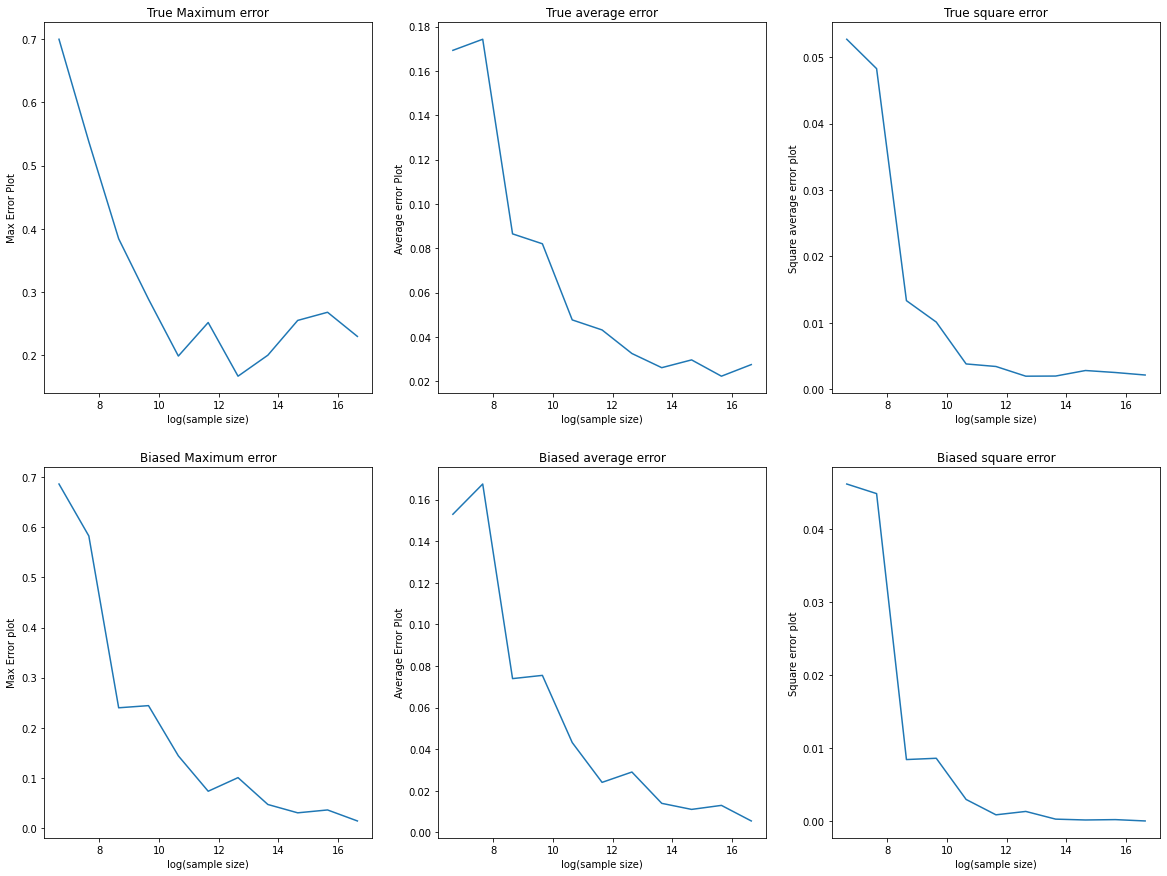
\includegraphics[width=0.95\textwidth]{gaussian_f_3_20_sim_better_bias_estimate.png}
    \caption{Error decay with sample size. The kernel is Gaussian $k(x,y)=\exp(-(\frac{x-y}{h})^2)$. The bandwith is set to $h=0.11$, the noise is set to $\sigma^2=1$, and the function to be estimated is $f(x)=2+x-e^{-x^2}$.
    The experiment is repeated 20 times and the average error curves are plotted.
    }
    \label{fig:error_decay}
\end{figure}

\begin{figure}
    \centering
    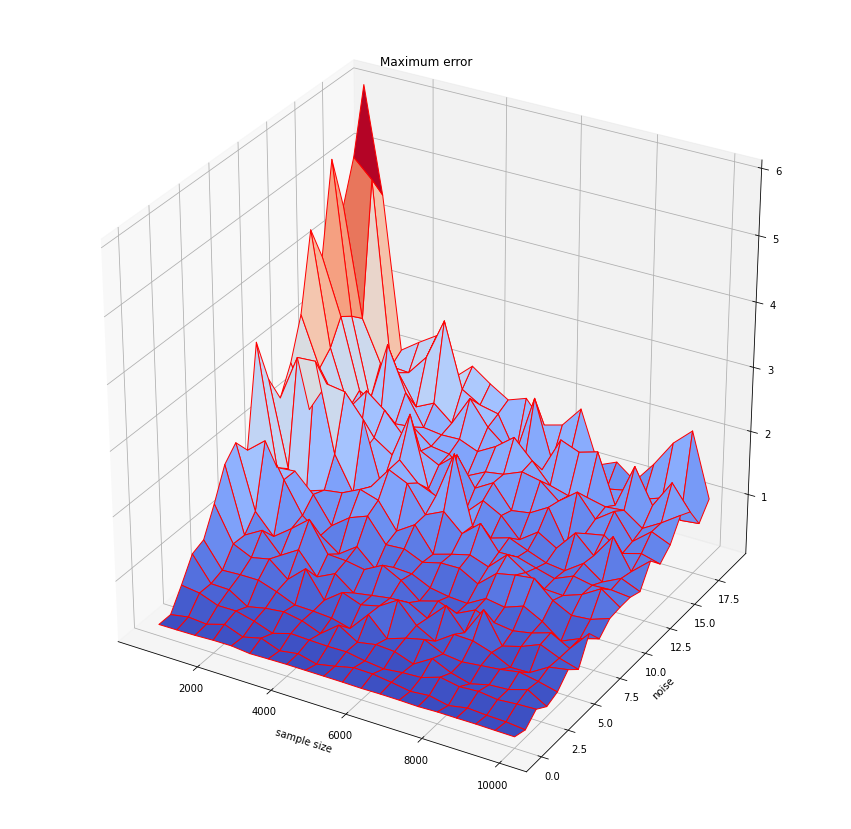
\includegraphics[width=0.65\textwidth]{gf3_noise_samplesize_coolwarm.png}
    \caption{True maximum error plotted against sample size and noise level. The parameters are as in Figure \ref{fig:error_decay}.}
    \label{fig:3d_plot}
\end{figure}


\subsection{ Estimating functions }
$\mathbb{P}$
$\mathbb{E}$
$\mathbb{a}$


\section{Appendix}

\subsection{related work/future plans}


Clustering algorithms on Stochastic block models 

\cite{Oliviera}


\cite{Lei_2015}


\cite{Levina-Vershynin}

Latent position model

\cite{Bickel}

\cite{Tang}

\cite{Arias-Castro}

\cite{Chatterjee}

\subsection{Probabilistic proof of the Bernoulli inequality}

The Bernoulli inequality\footnote{In fact the Bernoulli inequality states that for all $y>-1$ and $n\in\mathbb{N}$, $(1+y)^n\geq 1+ny$ but we are only interested in the case $-1<y<0$} states that for all $0<p<1$ and $n\in\mathbb{N}$, 
\begin{equation}
\label{bern_ineq}
    (1-p)^n\geq 1-np
\end{equation}
More generally, for $0<p<1$ and $n\in\mathbb{N}$ we are going to derive bounds for

\begin{equation}
\label{bin_remainder}
b_j=(-1)^j[(1-p)^n-\sum_{l=0}^{j-1}{n \choose l}(-1)^lp^l]
\end{equation}
The proof of Bernoulli's inequality follows easily from the 
observation that $R_1\leq 1$. Indeed, by Lemma \ref{lemma_exp}
\begin{equation*}
    \frac{1-(1-c(x))^n}{nc(x)}=ER_1\leq 1
\end{equation*}
Setting $p=c(x)$ one easily derives inequality (\ref{bern_ineq}). The following lemma provides bounds on 
(\ref{bin_remainder}).
\begin{lemma} For $j=1,2,...,n-1$
\begin{equation*}
    ER_{[j+1]}=\frac{1-jER_{[j]}}{(n-j)c(x)}
\end{equation*}

\end{lemma}
\begin{proof}
Using Equation (\ref{eqn_R}) for $l=j+1,...n$, we have

\begin{equation*}
    a(x,X_l)R_{[j]}=a(x,X_l)R_{[j]\cup\{l\}}
\end{equation*}
Summing these equations for $l=j+1,...,n$ we get

\begin{equation*}
\begin{split}
    1-jR_{[j]}&=1-\frac{j}{j+\sum_{l=j+1}^na(x,X_l)}\\
    &=\frac{\sum_{l=j+1}^n a(x,X_l)}{j+\sum_{l=j+1}a(x,X_l)}\\
    &=\sum_{l=j+1}^na(x,X_l)R_{[j]\cup\{l\}} 
\end{split}
\end{equation*}
Taking expectation and using the fact that $a(x,X_l)$ and $R_{[j]\cup\{l\}}$ are independent, and the fact that $R_{[j]\cup\{l\}}$ and $R_{[j+1]}$ are identically distributed, we get

\begin{equation*}
\begin{split}
    1-jER_{[j]}&=\sum_{l=j+1}^n Ea(x,X_l)R_{[j]\cup\{l\}}\\
    &=\sum_{l=j+1}^nEa(x,X_l)ER_{[j]\cup\{l\}}\\
    &=(n-j)c(x)ER_{[j+1]}
\end{split}    
\end{equation*}
\end{proof}

\begin{corollary}
For $j=1,2,3,...,n-1$ let $b_j$ be given by (\ref{bin_remainder}). Then 

\begin{equation*}
    \frac{j}{n}{n \choose j}p^j<b_j<{n\choose j}p^j
\end{equation*}
\end{corollary}

\begin{proof}
Consider the sequence $b^{'}_j=\frac{b_j}{j{n\choose j}p^j}$. It is easy to verify that $b^{'}_1=ER_1$ and that 

\begin{equation*}
    b^{'}_{j+1}=\frac{1}{1}
\end{equation*}

\end{proof}

\subsection{Alternative approach to concentration properties}
\subsubsection{Motivation and main ideas}

\paragraph{Motivation}
Given $x\in\mathbb{R}^d$, as soon as $c(x)>0$, the strong law of large numbers states that 

\begin{equation}
\label{bias_conv}
    \hat{f}_{GNW}(x)\rightarrow b(f,x) \textit{ almost surely}
\end{equation}

Although  statement (\ref{bias_conv}) is good as a heuristic, it is asymptotic in nature and hence of limited importance for theoretical guarantees such as sample complexities. We use concentration inequalities to specify a rate at which this convergence occurs. This section contains two results, one about concentration properties of $\hat{f}_{GNW}(x)$ with $x\in\mathbb{R}^d$ fixed and such that $c(x)>0$ and one about concentration properties of $\hat{f}_{GNW}(X)$ where $X,X_1,...,X_n$ are i.i.d. random variables with density $p$. We make the following assumptions throughout this section:

\begin{itemize}
    \item $f\colon\mathbb{R}^d\to\mathbb{R}$ is bounded and measurable with $||f||_{\infty}\leq B$
    \item $x\in\mathbb{R}^d$ is a point with $c(x)=\int k(x,z)p(z)dz>0$
    \item $X,X_1,...,X_n$ are i.i.d. random variables with density $p$
\end{itemize}

\paragraph{Concentration for a deterministic point}
The Graphical Nadaraya Watson estimator $\hat{f}_{GNW}(x)$ concentrates towards $b(f,x)$
for all bounded functions $f\colon \mathbb{R}^d\to \mathbb{R}$. The concentration is exponential in the number of samples $n$ and  depends on the parameter $c(x)=T_k(1)(x)=\int k(x,z)p(z)dz$. The precise statement of this result is Theorem \ref{thm_1}. The main idea in the proof is to show separately concentration for the statistics $\frac{1}{n}\sum_{i=1}^nY_ia(x,X_i)$ and $\frac{1}{n}\sum_{i=1}^n a(x,X_i)$ towards $T_k(f)(x)$ and $c(x)=T_k(f)(x)$ respectively.
The first step towards Theorem \ref{thm_1} is to show that $\frac{1}{n}\sum_{i=1}^n f(X_i)a(x,X_i)$ concentrates towards $\int f(z)k(x,z)p(z)dz$ using McDiarmid's concentration inequality. This is done in Lemma \ref{basic_lemma_1}. Next, we  need show that the noise term $\frac{1}{n}\sum_{i=1}^n\epsilon_ia(x,X_i)$ concentrates towards $0$. This is done in Lemma \ref{basic_lemma_2} using Subgaussian concentration inequalities. Finally, using Lemma \ref{basic_lemma_1} and Lemma \ref{basic_lemma_2} we prove Theorem \ref{thm_1}.

\paragraph{Concentration result for a random point} The situation is more involved in the case where $X$ is a random point. The first complications arise out of the fact that the variables $a(X,X_i)$ and $a(X,X_j)$ are no longer independent for $i\neq j$. The concentration  result in this case can be stated informally as
$\hat{f}_{GNW}(X)$ will concentrate towards $b(f,X)$ with a rate that is exponential in $n$ provided that the probability that $c(X)$ takes small values is small. The precise statement of this result is Theorem \ref{thm_2}. The first step towards the proof of Theorem \ref{thm_2} is to derive concentration statements about $\frac{1}{n}\sum_{i=1}^nY_ia(X,X_i)$ and $\frac{1}{n}\sum_{i=1}^n a(X,X_i)$ towards $T_k(f)(X)$ and $c(X)$ respectively. This is done in Corollary \ref{basic_cor_1} and Corollary \ref{basic_cor_2}, which can be considered as the random point analogues of Lemma \ref{basic_lemma_1} and Lemma \ref{basic_lemma_2} respectively. Informally speaking, one can think of Corollary \ref{basic_lemma_1} as integrating the inequality in Lemma \ref{basic_lemma_1} with respect to the density $p$.

\subsection{Concentration for a deterministic point}
\label{conc_det_pt}

\begin{lemma}
\label{basic_lemma_1}
Suppose that $f$ is bounded, measurable function with  $||f||_{\infty}\leq B$. Then 
\begin{equation*}
P(|\frac{1}{n}\sum_{i=1}^n f(X_i)a(x,X_i)-\int f(z)k(x,z)p(z)dz|\geq t)\leq 2\exp(-\frac{2t^2n}{5B^2})
\end{equation*}
\end{lemma}
\begin{proof} For $i=1,...,n$ we can write $a(x,X_i)=I(U_i\leq k(x,X_i))$ where $U_i$ are i.i.d. uniform  variables on $[0,1]$ independent from the $X_i's$ and $\epsilon_i's$. Define
\begin{equation*}
    F(x_1,...,x_n,u_1,...,u_n)=\frac{1}{n}\sum_{i=1}^n [f(x_i)I(u_i\leq k(x,x_i))-\int f(z)k(x,z)p(z)dz]
\end{equation*}
Note that $EF(X_1,...,X_n,U_1,...,U_n)=0$.
We will verify that $F$ satisfies the hypothesis of \\
McDiarmid's bounded difference inequality (\cite{vershynin} Thm 2.9.1). Changing one of the $x_i's$ gives:

\begin{equation*}
\begin{split}
    &|F(x_1,...,x_i,...,x_n,u_1,...,u_n)-F(x_1,...,x^{'}_i,...,x_n,u_1,...,u_n)|=\\
    &\frac{1}{n}|I(u_i\leq k(x,x_i))f(x_i)-I(u_i\leq k(x,x^{'}_i))f(x^{'}_i)|\leq \frac{2B}{n}
\end{split}
\end{equation*}

Changing one of the $u_i's$ gives:

\begin{equation*}
\begin{split}
        &|F(x_1,...,x_n,u_1,...u_i,...,u_n)-F(x_1,...,x_n,u_1,...u^{'}_i,...,u_n)|=\\
    &\frac{1}{n}|[I(u_i\leq k(x,x_i))-I(u^{'}_i\leq k(x,x_i))]f(x_i)|\leq \frac{B}{n}
\end{split}
\end{equation*}
Hence $F$ has the $(c_1,,,c_n,c_{n+1},...,c_{2n})$ bounded difference property with $c_1=c_2=...=c_n=\frac{2B}{n}$ and $c_{n+1}=...=c_{2n}=\frac{B}{n}$, giving $\sum_{i=1}^{2n}c_i^2=\frac{5B^2}{n}$. The result follows immediately from McDiarmid's inequality.
\end{proof}
In the following corollary we prove a concentration result for a variable $X$ which is independent and identically distributed with $X_1,...,X_n$.

\begin{lemma}
\label{basic_lemma_2}
Suppose that $w_1,...,w_n$ and $\epsilon_1,...,\epsilon_n$ are 
independent, $|w_i|\leq 1$ and $\epsilon_i$ are centered Gaussian variables with variance $\sigma^2$. Then

\begin{equation*}
    P(|\frac{1}{n}\sum_{i=1}^n w_i\epsilon_i|\geq t)\leq 2\exp(-\frac{3ct^2n}{8\sigma^2})
\end{equation*}

where $c>0$ is an absolute constant.
\end{lemma}
\begin{proof}
Consider the sub-gaussian norm of $w_1\epsilon_1$ defined as 

\begin{equation*}
    ||w_1\epsilon_1||_{\psi_2}=\inf\{t>0: E\exp(w_1\epsilon_1)^2/t^2)\leq 2\}
\end{equation*}
We have
\begin{equation*}
    E\exp( (w_1\epsilon_1)^2/t^2)\leq E\exp(\epsilon_1^2/t^2)=\frac{1}{\sqrt{1-\frac{2\sigma^2}{t^2}}}
\end{equation*}
as soon as $t$ is chosen such that $1-\frac{2\sigma^2}{t^2}>0$. Choosing $t= \sqrt{\frac{8\sigma^2}{3}}$ we get 

\begin{equation*}
    E\exp((w_1\epsilon_1)^2/t^2)\leq 2
\end{equation*}

In particular this shows that 

\begin{equation*}
    ||w_1\epsilon_1||_{\psi_2}^2\leq \frac{8\sigma^2}{3}
\end{equation*}

Using the General Hoeffding's inequality (\cite{vershynin} Thm 2.6.3), we have

\begin{equation*}
    P(|\frac{1}{n}\sum_{i=1}^n w_i\epsilon_i|\geq t)\leq 2\exp(-\frac{3ct^2n}{8\sigma^2})
\end{equation*}

with $c>0$ an absolute constant. 
\end{proof}
 
 
\begin{theorem}
\label{thm_1}
Suppose that $||f||_{\infty}\leq B$ and $c(x)=Ek(x,X_1)=\int k(x,z)p(z)dz>0$. Then
 for $0<\delta<3B$ and 
$H(B,\sigma^2)=\min\{\frac{1}{90B^2},\frac{C}{\sigma^2}\}$ we have

\begin{equation*}
    P(|\hat{f}_{GNW}(x)-\frac{\int f(z)k(x,z)p(z)dz}{\int k(x,z)p(z)dz}|\geq\delta)\leq 6\exp(-H(B,\sigma^2)c(x)^2\delta^2n)
\end{equation*}
\end{theorem}
\begin{proof} 
Let $\delta>0$ and denote

\begin{equation*}
\begin{split}
&A_{\delta}=\{|\frac{1}{n}\sum_{i=1}^n f(x_i)a(x,X_i)-\int f(z)k(x,z)p(z)dz|\geq \delta\}\\
&B_{\delta}=\{|\frac{1}{n}\sum_{i=1}^n a(x,X_i)-c(x)|\geq \delta\}\\
&C_{\delta}=\{|\frac{1}{n}\sum_{i=1}^n\epsilon_ia(x,X_i)|\geq \delta\}
\end{split}
\end{equation*}
Let $\delta_1, \delta_2,\delta_3>0$, we will  specify them later.
Choosing $\delta_2\leq\frac{1}{2}c(x)$, on $B_{\delta_2}^c$ we have
\\
$\frac{1}{n}\sum_{i=1}^na(x,X_i)\geq \frac{1}{2}c(x)$ and in particular $\sum_{i=1}^n a(x,X_i)>0$. Hence on $B_{\delta_2}^c$, we have 

\begin{equation}
\label{eqn:Equation_1}
\begin{split}
    \hat{f}_{GNW}(x)-\frac{\int f(z)k(x,z)p(z)dz}{c(x)}&=\frac{\frac{1}{n}\sum_{i=1}^nY_ia(x,X_i)}{\frac{1}{n}\sum_{i=1}^n a(x,X_i)}-\frac{\int f(z)k(x,z)p(z)dz}{c(x)}\\
    &=\frac{\frac{1}{n}\sum_{i=1}^n[f(X_i)-\frac{T_k(f)(x)}{c(x)}]a(x,X_i)}{\frac{1}{n}\sum_{i=1}^n a(x,X_i)}+\frac{\frac{1}{n}\sum_{i=1}\epsilon_ia(x,X_i)}{\frac{1}{n}\sum_{i=1}^n a(x,X_i)}
\end{split}
\end{equation}
In addition, on $(A_{\delta_1}\cup B_{\delta_2}\cup C_{\delta_3})^c$, we have
\begin{equation*}
\begin{split}
    |\hat{f}_{GNW}(x)-\frac{\int f(z)k(x,z)p(z)dz}{c(x)}|&\leq |\frac{\frac{1}{n}\sum_{i=1}^n[f(X_i)-\frac{T_k(f)(x)}{c(x)}]]a(x,X_i)}{\frac{1}{n}\sum_{i=1}^n a(x,X_i)}|+|\frac{\frac{1}{n}\sum_{i=1}\epsilon_ia(x,X_i)}{\frac{1}{n}\sum_{i=1}^n a(x,X_i)}|\\
    &= |\frac{\frac{1}{n}\sum_{i=1}^n [f(X_i)c(x)-T_k(f)]a(x,X_i)}{\frac{1}{n}c(x)\sum_{i=1}^na(x,X_i)}|+|\frac{\frac{1}{n}\sum_{i=1}\epsilon_ia(x,X_i)}{\frac{1}{n}\sum_{i=1}^n a(x,X_i)}|\\
    & = |\frac{c(x)[\frac{1}{n}\sum_{i=1}^nf(X_i)a(x,X_i)-T_k(f)(x)]+T_k(f)(x)[c(x)-\frac{1}{n}\sum_{i=1}^n a(x,X_i)]
    }{\frac{1}{n}c(x)\sum_{i=1}^na(x,X_i)}\\
    &+|\frac{\frac{1}{n}\sum_{i=1}\epsilon_ia(x,X_i)}{\frac{1}{n}\sum_{i=1}^n a(x,X_i)}|\\
    & \leq  \frac{c(x)(\delta_1+\delta_3)+T_k(f)(x)\delta_2}{\frac{1}{n}c(x)\sum_{i=1}^n a(x,X_i)}\\
    & \leq \frac{c(x)(\delta_1+B\delta_2+\delta_3)}{\frac{1}{n}c(x)\sum_{i=1}^n a(x,X_i)}\\
    & \leq \frac{2(\delta_1+\delta_2B+\delta_3)}{c(x)}
\end{split}
\end{equation*}
Finally, setting

\begin{equation*}
\delta_1=\delta_3=\frac{\delta c(x)}{6}, \textit{ } \delta_2=\frac{\delta c(x)}{6B}
\end{equation*}

we get 

\begin{equation*}
     |\hat{f}_{GNW}(x)-\frac{\int f(z)k(x,z)p(z)dz}{\int k(x,z)p(z)dz}|\leq \delta
\end{equation*}

on  $(A_{\delta_1}\cup B_{\delta_2}\cup C_{\delta_3})^c$.
\\
By Lemma \ref{basic_lemma_1}, we have $P(A_{\delta_1})\leq 2\exp(-\frac{2\delta_1^2n}{5B^2})$ and
$P(B_{\delta_2})\leq 2\exp(-\frac{2\delta_2^2n}{5})$.
\\
By Lemma \ref{basic_lemma_2} we have
$P(C_{\delta_3})\leq 2\exp(-\frac{C\delta_3^2n}{\sigma^2})$ where $C>0$ is a constant.

The result follows from a union bound 
\begin{equation*}
\begin{split}
    P(A_{\delta1}\cup B_{\delta_2}\cup C_{\delta_3})&\leq P(A_{\delta_1})+P(B_{\delta_2})+P(C_{\delta_3})\\
    &\leq 6\exp(-H(B,\sigma^2)c(x)^2\delta^2n)
\end{split}
\end{equation*}
\end{proof}

\subsection{Concentration for a random point}
\label{conc_random_pt}

\begin{corollary}
\label{basic_cor_1}
Suppose that $f$ is bounded, measurable function with $||f||_{\infty}\leq B$ and that $X,X_1,...,X_n$ are i.i.d. random variables with density $p$.
Then
\begin{equation*}
    P(|\frac{1}{n}\sum_{i=1}^nf(X_i)a(X_i,X)-\int f(z)k(X,z)p(z)dz|\geq t)\leq 2\exp(-\frac{2t^2n}{5B^2})
\end{equation*}
\end{corollary}
\begin{proof}
Let $U_1,...,U_n$ be i.i.d. uniform on $[0,1]$ such that $a(X,X_i)=I(U_i\leq k(X,X_i))$. Consider the indicator function $\phi:\mathbb{R}^{2n+1}\rightarrow\mathbb{R}$ given by 

\begin{equation*}
    \phi(x,x_1,...,x_n,u_1,...,u_n)=I(|\frac{1}{n}\sum_{i=1}^n f(x_i)I(u_i\leq k(x,x_i))-\int f(z)k(x,z)p(z)dz|\geq t)
\end{equation*}
According to \ref{basic_lemma_1}, we have

\begin{equation*}
\begin{split}
    E\phi(x,X_1,...,X_n,U_1,...,U_n)&= \int \phi(x,x_1,...,x_n,u_1,...,u_n)\prod_{i=1}^n p(x_i)\prod_{i=1}^n dx_i\prod_{i=1}^n du_i\\
    &=P(|\frac{1}{n}\sum_{i=1}^n f(X_i)a(x,X_i)-\int f(z)k(x,z)p(z)dz|\geq t)\\
    &\leq 2\exp(-\frac{2t^2n}{5B^2})
\end{split}
\end{equation*}
Finally, using Fubini's theorem, we have

\begin{equation*}
    \begin{split}
        P(|\frac{1}{n}\sum_{i=1}^nf(X_i)a(X_i,X)-\int f(z)k(X,z)p(z)dz|\geq t)&=E\phi(X,X_1,...,X_n,U_1,...,U_n)\\
        &=\int [\phi(x,x_1,..,x_n.u_1,...,u_n)\prod_{i=1}^n p(x_i)\prod_{i=1}^n dx_i\prod_{i=1}^n du_i]p(x)dx\\
        &=\int E\phi(x,X_1,...,X_n,U_1,...,U_n)p(x)dx\\
        &\leq 2\exp(-\frac{2t^2n}{5B^2})\int  p(x)dx\\
        &=2\exp(-\frac{2t^2n}{5B^2})
    \end{split}
\end{equation*}
\end{proof}

\begin{corollary}
\label{basic_cor_2}
Suppose that and $\epsilon_1,...,\epsilon_n$ are i.i.d. centered Gaussian variables with variance $\sigma^2$, $X,X_1,...,X_n$ are i.i.d. with density $p$. Then
 
 \begin{equation*}
    P(|\frac{1}{n}\sum_{i=1}^n \epsilon_ia(X,X_i)|\geq t)\leq 2\exp(-\frac{3ct^2n}{8\sigma^2})
 \end{equation*}
\end{corollary}
 \begin{proof}
 The result follows by Lemma  \ref{basic_lemma_2}  using the same method that was used to derive Corollary \ref{basic_cor_1} from Lemma \ref{basic_lemma_1}. 
 \end{proof}

\begin{theorem}
\label{thm_2}
Suppose that $||f||_{\infty}\leq B$ and 
$X,X_1,...,X_n$ are i.i.d. random variables 
with density $p$.
Set $H(B,\sigma^2)=\min(\frac{c_1}{\sigma^2},\frac{1}{90B^2})$. Then 
for all $r>0$ and $0<\delta<3B$ we have 

\begin{equation*}
    P(c(X)>0,|\hat{f}_{GNW}(X)-\frac{T_k(f)(X)}{c(X)}|\geq\delta)\leq 6\exp(-H(B,\sigma^2)r^2\delta^2n)+P(c(X)<r)
\end{equation*}

\end{theorem}

\begin{proof}

For $\delta,r>0$ and $f:\mathbb{R}^d\rightarrow \mathbb{R}$ bounded, let 
\begin{equation*}
    \begin{split}
        &C_r=\{\int k(X,z)p(z)dz\geq r\}=\{c(X)\geq r\}\\
        &A_{\delta}(f)=\{|\frac{1}{n}\sum_{i=1}^n f(X_i)a(X,X_i)-\int f(z)k(X,z)p(z)dz|\geq \delta\}\\
        &N_{\delta}=\{|\frac{1}{n}\sum_{i=1}^n \epsilon_ia(X,X_i)|\geq \delta\}
    \end{split}
\end{equation*}

Let $\delta_1,\delta_2,\delta_3>0$ to be specified later.
On $C_r\cap A_{\delta_1}(f)^c\cap A_{\delta_2
}(1)^c\cap N_{\delta}^c$ we have 

\begin{equation*}
    \frac{1}{n}\sum_{i=1}^n a(X,X_i)>c(X)-\delta_2\geq r-\delta_2\geq \frac{r}{2}
\end{equation*}
as soon as $\delta_2<\frac{r}{2}$. Furthermore the same calculation as in Theorem \ref{thm_1}
gives

\begin{equation*}
\begin{split}
     |\hat{f}_{GNW}(X)-\frac{\int f(z)k(X,z)p(z)dz}{c(X)}|&\leq \frac{\delta_1+\delta_3+\delta_2B}{\frac{1}{n}\sum_{i=1}^n a(X,X_i)}\\
     &\leq 2\frac{\delta_1+\delta_3+\delta_2B}{r}
\end{split}
\end{equation*}
Choosing $\delta_1=\delta_3=
\frac{r\delta}{6}$ and $\delta_2=\min(\frac{r}{2},\frac{r\delta}{6B})$, on $C_r\cap A_{\delta_1}(f)^c\cap A_{\delta_2
}(1)^c\cap N_{\delta}^c$ we have $c(X)>0$ and

\begin{equation*}
    |\hat{f}_{GNW}(X)-\frac{\int f(z)k(X,z)p(z)dz}{c(X)}|\leq \delta
\end{equation*}
To conclude, when $\delta<3B$, using Corollary \ref{basic_cor_1} and Corollary \ref{basic_cor_2} we have


\begin{equation*}
\begin{split}
    &P(c(X)>0,|\hat{f}_{GNW}(X)-\frac{T_k(f)(X)}{c(X)}|\geq\delta)\leq P(C_r^c\cup A_{\delta_1}(f)\cup A_{\delta_2
}(1)\cup N_{\delta})\\&\leq P(c(X)<r)+2\exp(-\frac{r^2\delta^2n}{90B^2})+2\exp(-\frac{r^2\delta^2n}{90B^2})+2\exp(-\frac{c_1r^2\delta^2n}{\sigma^2})\\
&\leq P(c(X)<r)+6\exp(-H(B,\sigma^2)r^2\delta^2n)
\end{split}
\end{equation*}

\end{proof}
\subsection{Remarks}

\begin{remark}
The quantity $H(B,\sigma^2)$ is inversly proportional to the boundedness and noise parameters $B$ and $\sigma^2$ respectively. In particular if either of the two parameters $B$ and $\sigma^2$ increases while the other is fixed, the quantity  $H(B,\sigma^2)=\min(\frac{C}{\sigma^2},\frac{1}{90B^2})$ decreases and hence the concentration rate in Theorem \ref{thm_1} and Theorem \ref{thm_2} decreases.
\end{remark}


\begin{remark}
The proof of Lemma \ref{basic_lemma_2} relies on sub-gaussian inequalities. These inequalities hold for a wider class of probability distributions, namely for subgaussian variables. Thus similar results hold if one assumes that the variables $\epsilon_i$ are i.i.d subgaussian.
\end{remark}

\begin{remark}
As long as $E|f(X_1)k(x,X_1)|=\int |f(z)|k(x,z)p(z)dz<\infty $ and $c(x)=\int k(x,z)p(z)dz>0$, the strong law of large numbers states that 

\begin{equation*}
    \hat{f}_{GNW}(x)\rightarrow \frac{\int f(z)k(x,z)p(z)dz}{\int k(x,z)p(z)dz}
\end{equation*}
This is the case if $E|f(X_1)|=\int f(z)p(z)dz<\infty$.
However, it is not clear how to obtain concentration results for such a weak assumption. Under weaker assumption such as $f(X_1)\in L^2$ one can use Chebyshev or Markov inequalities to find a concentration rate.  One way to slightly generalize the function class (while preserving the strong concentration rate) is to consider functions $f$ for which $f(X_1)$ is sub-gaussian i.e. there exists $t>0$ such that 

\begin{equation*}
    E\exp(\frac{f^2(X_1)}{t^2})=\int \exp(\frac{f^2(z)}{t^2})p(z)dz<\infty  
\end{equation*}

With such an assumption on $f$ it is possible to replace McDiarmid's bounded difference inequality with Hoeffding's inequality to obtain similar concentration result, where the constant $B$ is replaced by an upper bound of the $\psi_2$ subgaussian norm $\psi_2(X_1)$
\end{remark}

\begin{remark} A slight modification of the presented proofs shows that the classical Nadaraya Watson estimator $\hat{f}_{NW}$ given by \ref{NW_def} satisfies 
\begin{equation*}
    P(|\hat{f}_{GNW}(x)-\hat{f}_{NW}(x)|\geq \delta)\leq c_1\exp(-H_1(B,\sigma^2)c(x)^2\delta^2n)
\end{equation*}
for some absolute constants $c_1>0$ and $H_1(B,\sigma^2)>0$.
Indeed, if we take
\begin{equation*}
    F_1(x_1,...x_n)=\frac{1}{n}\sum_{i=1}^n [f(x_i)k(x,x_i)-\int f(z)k(x,z)p(z)dz]
\end{equation*}
then $EF_1(X_1,...,X_n)=0$ and similar ideas as in Lemma \ref{basic_lemma_1} apply. We omit the details. Note that the ambient space in which the data  $X_1,...,X_n$ is embedded does not a play a role in this section as long as the variables are independent and $||f||_{\infty}\leq B$. In particular the dimensionality of the data plays no role in the approximation of $\hat{f}_{NW}$ by $\hat{f}_{GNW}$. However, we still have to take into account that our ultimate goal is to estimate $f$, and not $\hat{f}_{NW}$, and the dimensionality of the data will play an important role here as we show in the next section.
\end{remark}




\begin{remark}
Assuming that $\inf_{x\in\supp{p}} c(x)\geq r>0$ gives $P(\int k(X,z)p(z)dz<r)=0$ so that by Theorem \ref{thm_2}, $\hat{f}_{GNW}(X)$ concentrates around $\frac{\int f(z)k(X,z)p(z)dz}{\int k(X,z)p(z)dz}$ with exponentially small probability in the sample size $n$. An application of Borel-Cantelli's lemma in such a case gives that $\hat{f}_{GNW}(X)\rightarrow \frac{T_k(f)(X)}{T_k(1)(X)}$ almost surely. This is the case For example $p(z)$ is compactly supported density (i.e. the data $X_1,...,X_n$ are drawn i.i.d. from some compact set) and $c(x)>0$ for all $x$ in the support of $p$. In general, there is a penalty term $P(\int k(X,z)p(z)dz<r)$ which is highly dependent on the kernel $k$. However it is still true that $\hat{f}_{GNW}(X)$ converges in probability towards $\frac{\int f(z)k(X,z)p(z)dz}{c(X)}$.
\end{remark}


\subsection{A Generalization: Higher order GNW estimators}

In this section we discuss a generalization of the Graphical Nadaraya Watson which averages the observations $Y_i$ over vertices which have fixed graph distance $m$ from $X$. Using Corollary 1 we show that this estimator concentrates around the quantity $\frac{T_k^m(f)(X)}{c_m(X)}$ with probability 

\subsubsection{Second order GNW estimator \texorpdfstring{$\hat{f}_{GNW,m}$}{Lg}}

The proposed estimator $\hat{f}_{GNW}$ does not take advantage of the graph structure of the data. The estimator at a vertex
$v$ is based only on neighbours of 
$v$. In order to account for the potential influence of vertices which are not direct neighbours of $v$, we introduce the weights\footnote{ At this point we have not stated anything about self edges in the observed graph. As long as the variables $a(X_i,X_i)$ are
bounded and 
independent, their contribution will vanish for large n so to simplify the exposition we assume that $a(X_i,X_i)=0$.
}


\begin{equation*}
    w_{2}(X_i,X)=\sum_{j=1,j\neq i}^na(X_i,X_j)a(X_j,X)
\end{equation*}

We introduce the \textbf{Second order GNW estimator}:

\begin{equation*}
    \hat{f}_{GNW,2}(x)=\frac{\sum_{i=1}^n Y_i
    w_2(X_i,x)}{\sum_{i=1}^n w_2(X_i,x)}
\end{equation*} 
\paragraph{Lemma 6} Suppose that $||f(X_1)||_{\infty}\leq B$, and $X,X_1,...,X_n$ are i.i.d. with density $p$. Then

\begin{equation*}
     P(|\frac{1}{n(n-1)}\sum_{i=1}^n f(X_i)w_2(X_i,X)-T_k^2(f)(X)|\geq 2\delta)\leq (2n+2)\exp(\frac{-2\delta^2(n-1)}{5B})
\end{equation*}

\begin{proof}
Set 

\begin{equation*}
    S_j=\frac{1}{n-1}\sum_{i\neq j}f(X_i)a(X_i,X_j)
\end{equation*}

We compute:

\begin{equation}
\label{eqn:Equation_4}
\begin{split}
    \frac{1}{n(n-1)}\sum_{i=1}^n f(X_i)w_2(X_i,X)&
    =\frac{1}{n(n-1)}\sum_{j=1}^n[\sum_{i\neq j} f(X_i)a(X_i,X_j)]a(X_j,X)\\
    &=\frac{1}{n}\sum_{j=1}^n [\frac{1}{n-1}\sum_{i\neq j} f(X_i)a(X_i,X_j)-\int f(z)k(X_j,z)p(z)dz]a(X_j,X)\\
    & +\frac{1}{n}\sum_{j=1}^n[\int f(z)k(X_j,z)p(z)dz]a(X_j,X)\\
    &=\frac{1}{n}\sum_{j=1}^n [S_j-T_k(f)(X_j)]a(X_j,X)+\frac{1}{n}\sum_{j=1}^n T_k(X_j)a(X_j,X)
\end{split}
\end{equation}

Given $1\leq j\leq n$, according to Corolary 1 applied to the $n-1$ variables $X_1,...,X_{j-1},X_{j+1},...,X_n$, we have
\begin{equation*}
P(|S_j-T_k(f)(X_j)|\geq \delta)\leq 2\exp(-\frac{2\delta^2(n-1)}{5B})
\end{equation*}
Hence, by a union bound we have 
\begin{equation*}
\begin{split}
    P(|\frac{1}{n}\sum_{j=1}^n [S_j-T_k(f)(X_j)]a(X_j,X)|\geq\delta)
    )&\leq \sum_{i=1}^n P(|S_j-T_k(f)(X_j)|\geq \delta)\\
    &\leq 2n\exp(-\frac{2\delta^2(n-1)}{5B})
\end{split}
\end{equation*}
Applying Corolary 1 with $f_1(x)=T_k(f)(x)=\int f(z)k(x,z)p(z)dz$ (which is also bounded by $B$), we have

\begin{equation*}
    P(|\frac{1}{n}\sum_{j=1}^nT_k(f)(X_j)
    a(X_j,X)-T_k^2(f)(X)|\geq \delta)\leq 2\exp(-\frac{2\delta^2n}{5B})
\end{equation*}
Finally, combining the last two displays together with (\ref{eqn:Equation_4}), we have
\begin{equation*}
\begin{split}
    P(|\frac{1}{n(n-1)}\sum_{i=1}^n f(X_i)w_2(X_i,X)-T_k^2(f)(X)|\geq 2\delta)&\leq P(|\frac{1}{n}\sum_{j=1}^n [S_j-T_k(f)(X_j)]a(X_j,X)|\geq\delta)\\& +P(|\frac{1}{n}\sum_{j=1}^nT_k(f)(X_j)
    a(X_j,X)-T_k^2(f)(X)|\geq \delta)\\
    &\leq (2n+2)\exp(-\frac{2\delta^2(n-1)}{5B})
\end{split}
\end{equation*}
\end{proof}
\paragraph{Theorem 4} For any $r>0$, 
\begin{equation*}
  P(|\hat{f}_{GNW,2}(X)-\frac{T_k^2(f)(X)}{c_2(X)}|
   \geq \frac{(4r+2)\delta}{r^2})\leq P(c_2(X)<r)+c_1n\exp(-H(B,\sigma^2)\delta^2(n-1))
\end{equation*}
\begin{proof}
Denote 
\begin{equation*}
\begin{split}
    &C_r=\{c_2(X)\geq r\}=\{\int\int k(X,w)k(w,z)p(w)p(z)dwdz\geq r\}\\
    &A_{\delta}(f)=\{|\frac{1}{n(n-1)}\sum_{i=1}^n f(x_i)w_2(x,X_i)-T_k^2(f)(X)|\geq \delta\}\\
    &N_{\delta}=\{|\frac{1}{n(n-1)}\sum_{i=1}^n \epsilon_i w_2(X_i,X)|\geq \delta\}
\end{split}
\end{equation*}
As soon as $\delta<\frac{r}{2}$, on $C_r\cap A_{\delta}(1)^c$ we have
\begin{equation*}
    \begin{split}
        \hat{f}_{GNW,2}(X)
        &=\frac{\frac{1}{n(n-1)}\sum_{i=1}^n f(X_i)w_2(X_i,X)-T_k^2(f)(X)}{\frac{1}{n(n-1)}
        \sum_{i=1}^n w_2(X,X_i)}\\
        &+\frac{
        T_k^2(f)(X)}{\frac{1}{n(n-1)}\sum_{i=1}^n w_2(X_i,X)}+\frac{\sum_{i=1}^n \epsilon_iw_2(X_i,X)}{\sum_{i=1}^n w_2(X_i,X)}
    \end{split}
\end{equation*}
and 
\begin{equation*}
    \frac{1}{\frac{1}{n(n-1)}w_2(X_i,X)}\leq \frac{2}{r}
\end{equation*}
In particular $\hat{f}_{GNW,2}(X)$ is well defined on $C_r\cap A_{\delta}(1)^c$ 

Using the same technique as in Lemma 6, together with subgaussian concentration inequalities we can show that\footnote{ The technical details can be provided later if necessary}

\begin{equation*}
    P(|\frac{1}{n(n-1)}\sum_{i=1}^n \epsilon_i w_2(X_i,X)|\geq \delta)\leq c_1n\exp(-C(\sigma^2)\delta^2(n-1)) 
\end{equation*}
where $c_1,C(\sigma^2)>0$.
\\
On $C_r\cap A_{\delta}(1)^c\cap A_{\delta}(f)^c$ we have

\begin{equation*}
    \begin{split}
    |\frac{\frac{1}{n(n-1)}\sum_{i=1}^n f(X_i)w_2(X_i,X)-\int \int f(z)k(w,z)k(w,X)p(z)p(w)dzdw
    }{\frac{1}{n(n-1)}
    \sum_{i=1}^n w_2(X,X_i)}|&\leq \frac{2\delta}{r}
    \end{split}
\end{equation*}
Next, on $C_r\cap A_{\delta}(1)^c$ we have 
\begin{equation*}
    |\frac{1}{\frac{1}{n(n-1)}\sum_{i=1}^n w_2(X_i,X)}
    -\frac{1}{\int\int k(X,z)k(z,w)p(z)p(w)dzdw}|\leq \frac{2}{r^2}\delta
\end{equation*}
Finally, 
on $C_r\cap A_{\delta}(1)^c\cap A_{\delta}(f)^c\cap N_{\delta}^c$ we have

\begin{equation*}
    \begin{split}
         |\hat{f}_{GNW,2}(X)-\frac{T_k^2(f)(X)}{c_2(X)}|\leq \frac{4\delta}{r}+\frac{2\delta}{r^2}
    \end{split}
\end{equation*}
We conclude with a union bound
\begin{equation*}
    P(C_r^c\cup A_{\delta}(1)\cup A_{\delta}(f)\cup N_{\delta})\leq P(C_r^c)+c_1n\exp(-H(B,\sigma^2)\delta^2(n-1))
\end{equation*}
\end{proof}
\paragraph{Corollary 4} If $r=\inf_{x\in \supp p} c_2(x)>0$ then

\begin{equation*}
   P(|\hat{f}_{GNW,2}(X)-\frac{T_k^2(f)(X)}{c_2(X)}|
   \geq \frac{(4r+2)\delta}{r^2})\leq c_1n\exp(-H(B,\sigma^2)\delta^2(n-1))
\end{equation*}
\begin{proof}
Follows immediately from Theorem 3.
\end{proof}

\paragraph{Remarks}

\paragraph{Remark 8 (Higher order GNW Estimators)}
Given $1\leq m\leq n$, we introduce the weights

\begin{equation*}
    w_m(X_i,X)=\sum_{J_{i}} \prod_{j=0}^{m-1} a(X_{i_j},X_{i_{j+1}})
\end{equation*}
Here, $J_{i}=(i,i_1,...,i_{m-1})$ is a $m$-tuple of distinct indicies with the convention that
$i_0=i$ and $X_{i_m}$ is identified with $X$ and the sum is taken over all such $m$-tuples $J_i$. We introduce the \textbf{GNW estimator of order m}:
\begin{equation*}
    \hat{f}_{GNW,m}(X)=\frac{\sum_{i=1}^n Y_iw_m(X_i,X)}{\sum_{i=1}^n w_m(X_i,X)}
\end{equation*}
The case $m=2$ which was discussed in the previous paragraph is can be used as an inductive step in proving a concentration inequality for $\hat{f}_{GNW,m}$. It can be shown in a simmilar manner in which Lemma 6 was shown that 

\begin{equation*}
P(|\frac{(n-m)!}{n!}\sum_{i=1}^n f(X_i)w_m(X_i,X)-\frac{(n-(m-1))!}{n!}\sum_{i=1}^n T_k(f)(X_i)w_{m-1}(X_i,X)|\geq \delta)\leq 2n^{m-1}\exp(-\frac{2\delta^2(n-(m))}{5B})
\end{equation*}
\paragraph{Remark 9 (Application to the Stochastic Block Model)} The stochastic block model $SBM(n,W,p)$ (where $n$ is a positive integer, $W$ a $k\times k$ symmetric matrix with entries in $[0,1]$ and
$p=(p_1,...,p_k)$ is such that
$p_1+...+p_k=1$ and $p_i>0$, $i=1,...,n$)
is a random graph model that can be defined as follows:
Each node $i$ belongs to one of $k$
(disjoint) sets $B_1,...,B_k$ independently from the other nodes $j\neq i$ and with $P(i\in B_l)=p_k$, 
$1\leq l \leq k$. Then for any two blocks $B_l, B_s$,  we have

\begin{equation*}
    P(i\sim j|i\in B_l,j\in B_s)=W_{l,s}
\end{equation*}
The nodes $1,2,....,n$ may be thought of as individuals, the sets $B_l$ may be thought of as different blocks or communities and the parameters $W_{l,s}$ as the probability of connection between blocks $B_l$ and $B_s$. The Stochastic block model is a special case of Latent position model. Indeed, 
p to be a uniform $[0,1]$ distribution with kernel 

\begin{equation*}
    k(x_{i},x_{j})=\sum_{l\leq s} W_{l,s} I(x_{i}\in B_l, x_{j}\in B_s)
\end{equation*}

where $B_l$ is the semi-open interval with endpoints $\sum_{j=1}^{l-1}p_j$ and $\sum_{j=1}^{l}p_j$.
Then it is easy to see that the probability of edge between two vertices $i,j$ 
in this Latent position model is equal to the probability of edge between the vertices $i,j$ in a Stochastic block model $SBM(n,W,p)$. From here 
and the previous remark 
it follows that edge related statistics such as $w_m(i,j)$ can identyify the individuals in blocks with high probability, under suitable  assumptions that these statistics differ among blocks. We omit the details.



\section{maybe useful?}
As $pdx$ is a probability measure, compositions of $T_k$ of any order
$m\geq 1$
are well defined, and 

\begin{equation*}
    T_k^m(f)(x)=\int_{\mathbb{R}^d} T_k^{m-1}(f(z))k(x,z)p(z)dz
\end{equation*}

\paragraph{ remarks? }
 If $\int ||y||^2k(y)dy<\infty$,
    $p$ is $\beta$ Holder continuous, with $0<\beta\leq 1$ and $p(x)>0$ then there exists $n(x)\in \mathbb{N}$ such that for all $n\geq n(x)$,
    \begin{equation*}
        |\frac{T_{k_n}(f)(x)}{T_{k_n}(1)(x)}-f(x)|\leq ch_n^{\alpha}
    \end{equation*}
    with $c>0$ an absolute constant depending on $k$ and the Holder constants of $f$ and $p$.
\paragraph{remarks..}
\begin{itemize}
    \item Suppose now that $k$ is compactly supported and let $M>0$ be a constant such that $k(x)=0$ for $|x|>M$. Then, from (\ref{eqn:bias}) we get 
\begin{equation*}
    |\frac{T_{k_n}(f)(x)}{T_{k_n}(1)(x)}-f(x)|\leq LM^{\alpha}h_n^{\alpha}
\end{equation*}
This bound is independent of $x\in\supp{p}$ and of $f$ in the Holder class, and this proves the first claim.
    \item Now suppose $p(x)>0$ and $p$ is $\beta$-Holder continuous. Then for any $G(y)$ such that both 
    $\int |G(y)|k(y)dy<\infty$ and $\int ||y||^{\beta}|G(y)|k(y)dy<\infty$ we have
    \begin{equation}
    \
    \begin{split}
        |\int G(y)k(y)p(x+h_ny)dy-p(x)\int G(y)k(y)dy|&=|\int G(y)k(y)[p(x+h_ny)-p(x)]dy|\\
        &\leq h_n^{\beta}\int ||y||^{\beta}|G(y)|k(y)dy
    \end{split}
    \end{equation}
    In particular, for $G(y)=||y||^{\alpha}$ and $G(y)=1$ we get that for $n$ sufficiently large (potentially depending on $x$)
    
    \begin{equation*}
        \int ||y||^{\alpha}k(y)p(x+h_ny)dy\leq c_1 p(x)
    \end{equation*}
    
    and
    
    \begin{equation*}
        \int k(y)p(x+h_ny)dy\geq c_2p(x)
    \end{equation*}
    where $c_1,c_2>0$ depend on $k$ and the Holder constants of $p$.
    Hence, using these estimates in (\ref{eqn:bias}), we get
    
    \begin{equation*}
        |\frac{T_{k_n}(f)(x)}{T_{k_n}(1)(x)}-f(x)|\leq ch_n^{\alpha}
    \end{equation*}
    where $c>0$ is an absolute constant depending on $k$ and the Holder constants of $f$ and $p$.
\end{itemize}

\paragraph{suboptimal stuff} \paragraph{Lemma 4} Suppose that $p$ is $\beta$-Holder continuous, i.e. there is an $L>0$ such that for all $x,z\in\mathbb{R}^d$
\begin{equation*}
    |p(x)-p(z)|\leq L||x-z||^{\beta}
\end{equation*}
Suppose also that $p(x)>0$.
\begin{itemize}
    \item if $\lambda_nh_n^d=\omega(\frac{1}{\sqrt{n}})$
    then $\hat{f}_{GNW}(x)\rightarrow f(x)$ in probability.
    \item if $\lambda_nh_n^d=\omega(\sqrt{\frac{\log{n}}{n}})$
    then $\hat{f}_{GNW}(x)\rightarrow f(x)$ almost surely.
\end{itemize}
\begin{proof}
We begin by observing that $c_n(x)=T_{k_n}(1)(x)$ is important in the concentration of $\hat{f}_{GNW}$. In order to keep the concentration property we need to have


\begin{equation}
\label{eqn:equation_3}
    \lim_{n\rightarrow\infty} c_n(x)^2n=\infty
\end{equation}
We recall the expression
\begin{equation*}
    c_n(x)=\lambda_n\int k(\frac{x-z}{h_n})p(z)dz=\lambda_n h_n^d \int k(y)p(x+h_ny)dy
\end{equation*}
Using the $\beta$-Holder assumption on $p$, we have 
\begin{equation*}
\begin{split}
    |\lambda_n^{-1}h_n^{-d}c_n(x)-p(x)\int k(y)dy|&=|\int k(y)[p(x+h_ny)-p(x)]dy|\\
    &\leq \int k(y)|p(x+h_ny)-p(x)|dy\\
    &\leq Lh_n^{\beta}\int ||y||^{\beta}k(y)dy
\end{split}
\end{equation*}
From here it is easy to see that there are $c_1,c_2>0$ such that for $n$ sufficiently large
(potentially depending on $x$), 

\begin{equation}
\label{eqn:degree_bounds}
    c_1p(x)
    \lambda_nh_n^d\leq c_n(x)\leq c_2p(x) \lambda_nh_n^d
\end{equation}
\begin{itemize}
    \item  Suppose that $\lambda_nh_n^d=\omega(\frac{1}{\sqrt{n}})$. Then using Theorem 1 and \ref{eqn:degree_bounds} we get that $\hat{f}_{GNW}(x)\rightarrow f(x)$ as $n\rightarrow\infty$.
    \item Suppose that $\lambda_nh_n^d=\omega(\sqrt{\frac{\log{n}}{n}})$. Then for $n$ sufficiently large,  $\exp(-c_1\lambda_n^2h_n^{2d}n)\leq n^{-(1+r)}$ and hence by Borel-Cantelli lemma, 
    \begin{equation*}
        \hat{f}_{GNW}(x)-\frac{T_{k_n}(f)(x)}{T_{k_n}(1)(x)}\rightarrow 0 \textit{ almost surely as } n\rightarrow\infty
    \end{equation*}
   Now the result follows from Lemma 3 (which is a deterministic statement).
\end{itemize}
\end{proof}



\printbibliography
\nocite{*}






\end{document}

%%% Local Variables:
%%% mode: latex
%%% TeX-master: t
%%% End:
